\documentclass{polytech/polytech}
\usepackage{tikz}
%\usepackage[backend=biblatex]{biblatex}
%\usepackage{cite}

%-----------Configuration du rapport-----------------

\schooldepartment{peip}
\typereport{peip2}
\reportyear{2016-2017}
\title{DI 6 Correcteur de posture assise à base d'Arduino}
\reportlogo{image/logo_1ere_couverture} %A changer avec la photo de 1ere de couverture
\student{Jérémy}{LOCHE}{jeremy.loche@etu.univ-tours.fr}
\student{Dimitrios}{KOKKONIS}{dimitrios.kokkonis@etu.univ-tours.fr}
\academicsupervisor[di]{Sébastien}{BEAUFILS}{sebastien.beaufils@univ-tours.fr}

%------------Poster------------------

\posterblock{Test de l'application Android avec un sac}{Pour tester l'application Android, on a posé un sac sur une chaise à quatre pieds; puis on s'est connecté par Bluetooth pour visualiser le déplacement du centre de gravité du sac.}{image/poster_1}{Test du correcteur de posture en déplaçant un sac sur une chaise}

\posterblock{Preséntation du montage}{Le correcteur de posture comporte quatre cellules de charge, quatre amplificateurs HX711 et un Arduino UNO avec son Shield Bluetooth. Ici, nous l'avons alimenté par un \textit{powerbank}, et on s'est connecté à l'Arduino par Bluetooth avec l'application Android qu'on a construit pour visualiser le correcteur de posture.}{image/poster_2}{Le montage électronique de notre correcteur de posture}

\posterblock{Titre 3 poster}{texte 3 poster}{image/poster_3}{légende 3 poster}




%------------------Résumés & mots clés------------

\resume{Ce projet a pour but de créer un correcteur de posture assise d'une personne, sous la forme d'un système embarqué. Le projet est basé sur un Arduino Uno, qui gère les données de quatre capteurs de charges placées sous les pieds d'une chaise. On l'utilise ensuite pour transmettre ces données en série (soit par Bluetooth, soit par USB) à une application fonctionnant sur un ordinateur Windows/OSX/Linux ou un appareil Android. Cette application permet de visualiser la chaise, la position du barycentre de l'utilisateur dans une zone de confort calibrée par l'utilisateur.  On peut ainsi détecter si la posture de l'utilisateur est bonne; l'application l'informe visuellement quand ce n'est pas le cas. Le logiciel utilisé est écrit en Java et en C.}



\abstract{This project aims to create an application for correcting one's sitting posture, using both software and hardware. The project was built upon an Arduino Uno that handles the data sent by four load sensors placed under the feet of a chair, and which in turn modifies and sends that data in serial form (either by Bluetooth or by USB) to an application that runs on a Windows/OSX/Linux computer or an Android device. That device then provides the user with a graphic representation of the chair, the barycenter of the user, as well as a "deadzone" which is calibrated by the user, and is used to detect wether the user's posture is incorrect or not; the application informs the user visually when he is not properly seated. The software is written in Java and C.}


\motcle{Correction de posture, Système embarqué, Arduino, Java, C}

\keyword{Posture correction, Embedded system, Arduino, Java, C}


\addbibresource{biblio.bib}

\begin{document}


\chapter*{Introduction}

De nos jours\citation{article}, de nombreuses personnes souffrent du mal de dos dut à une mauvaise posture assise. En effet, il suffit de se rendre dans une salle de cours pleine d'étudiants pour constater que beaucoup d'entre eux sont mal assis. C'est pourquoi, nous avons choisi de travailler sur le projet de développement d'un correcteur de posture assise proposé par M.Beaufils. La proposition de M. Beaufils a été de construire ce dispositif à partir d'un Arduino Uno et des capteurs de forces placés sous les pieds d'une chaise. 

Le but de ce rapport va donc être de vous aider à comprendre comment on peut exploiter des capteurs de forces et un dispositif de type micro-contrôleur pour déterminer la qualité de l'assise. 

Ce projet s'articulant sur deux grands axes, matériel et logiciel, nous aborderons ces deux thématiques.
Nous discuterons, dans un premier temps, comment il est possible de déterminer la posture d'une personne. Nous en profiterons pour passer en revue les étapes de réalisation d'un dispositif capable de réaliser cette fonction. Pour illustrer brièvement cette partie, nous parlerons de capteurs de forces, de micro-contrôleur et de circuits électriques permettant d'implémenter cette fonction.

Dans un second temps, nous parlerons de l'aspect logiciel de ce projet venant se greffer sur le dispositif matériel. Pour vous donner un avant-goût du contenu de cette partie, nous aborderons la programmation du micro-contrôleur, et l'élaboration d'une application PC et Android permettant la visualisation des données des capteurs de manière compréhensible pour l'utilisateur.
Nous discuterons de l'organisation du développement informatique, et vous parlerons des outils que nous avons utilisés.


Comme vous l'avez compris, ce rapport vous permettra d'avoir le loisir de découvrir notre projet. Vous comprendrez alors le choix du matériel utilisé, la solution logicielle que nous proposons et les contraintes de réalisations aussi bien logicielles que matérielles auxquelles nous avons dut faire face.


\textbf{Transisition:} Sans plus attendre, entrons dans le vif du sujet en commençant par répondre à la question :

\begin{center}
\textit{Comment déterminer la posture assise d'une personne ? }
\end{center}

\chapter{Un correcteur de posture assise ? Qu'est ce que c'est ?}
\label{chap:correcteur posture}

Un correcteur de posture assise, telle que nous l'interprétons dans ce projet, est un dispositif qui permet à l'utilisateur de savoir s'il est bien assis où non. Il y a donc deux questions qui se posent assez naturellement:

\begin{enumerate}
\item Comment détermine-t-on la posture d'une personne ?
\item Comment montrer à l'utilisateur la qualité de son assise ?
\end{enumerate}

Ce chapitre du rapport sera consacré à la réponse que nous proposons à la première question et le chapitre suivant sera consacré à la seconde question.

\section{Déterminer la posture d'une personne}
\label{chap:posture_determination}

Pour déterminer la position assise d'une personne, nous avons proposé de récupérer les informations des forces appliqués aux niveau des pieds de la chaise. 

L'idée ici est d'utiliser la projection du centre de masse sur le sol pour déterminer la qualité de l'assise. 

\begin{center}
\textit{Comment ça marche concrètement ? Pourquoi mesure-t-on la force au niveau des pieds de la chaise ?} 
\end{center}

Lorsque l'on est assis sur une chaise, on exerce une force (le poids) qui est transférée au sol par les pieds de celle-ci. En effet, la force totale appliquée sur la chaise est répartie intégralement sur les pieds.

La répartition des forces n'est pas homogène et dépend de l'assise. C'est essentiellement ce principe que nous utilisons pour déterminer la qualité de l'assise d'une personne. C'est cette hétérogénéité dans la répartition des masses que nous allons quantifier.

La figure \ref{fig:illustr_chaise_forces}  illustre la répartition des forces pour différentes assises.

\begin{figure}[htbp]
\begin{center}
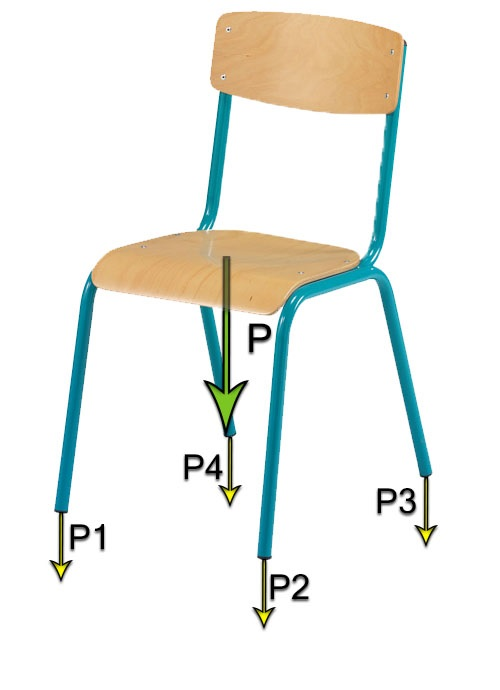
\includegraphics[scale=1]{image/Chaise_forces_homo.jpg}
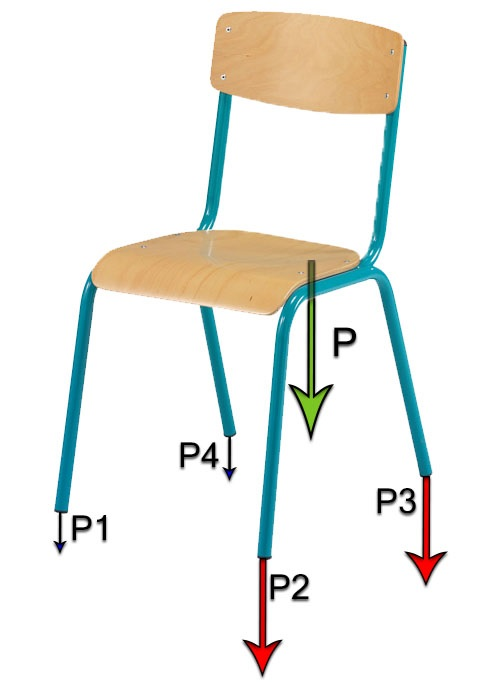
\includegraphics[scale=1]{image/Chaise_forces_hetero.jpg}
\end{center}
\caption{Illustration de la projection de la résultante des forces appliqués à la chaise vue au niveau des pieds de celle-ci pour deux position assises différentes.}
\label{fig:illustr_chaise_forces}
\end{figure}

En pratique, on ne connais pas l'emplacement du point d'application de la force sur le plateau de la chaise. Or c'est déterminer sa position qui permet de définir la qualité de l'assise. Une bonne assise donnera une répartition des masses donnée et donc une position de la force totale donnée. Par exemple dans la figure \ref{fig:illustr_chaise_forces}, l'image de gauche correspond à quelqu'un qui serait assis bien droit au centre de la chaise tandis que l'image de droite correspond à quelqu'un assis (ou penché) du coté gauche de la chaise.

Cependant, connaissant la position de chaque pieds, et connaissant la valeur de la force appliquée à chaque pied, on peut trouver la position du barycentre des forces (c'est à dire, la position de la force totale et donc celle du centre de masse). 

Nous allons voir comment résoudre ce problème. Nous rappelons que le but est de déterminer la position du centre de masse, caractéristique de la posture.

Ici on considère le poids (c'est à dire les forces liés à la masse). Le barycentre des forces obtenus correspond donc au centre de masse. 
Par la suite, nos calculs se feront en 2 dimensions dans le plan du sol. En effet, on assimile les pieds de la chaise à des points du plan. On place un point $O$ origine du repère dans le plan. 

Pour chaque pieds de la chaise on associe les grandeurs suivantes:

\begin{enumerate}
\item un numéro $i$
\item un point du plan $A_i=(x,y)$ avec $x,y$ ses coordonnées
\item une valeur de force notée $m_i$ (par analogie à la masse)
\item un vecteur position $\vec{OA_i}$ représentant la position du point par rapport au point $O$
\end{enumerate}

L'idée ici est de représenter la chaise dans le plan du sol. La figure \ref{fig:schem_plan_sol_math} illustre une chaise carrée dont les quatre pieds sont projetés dans le plan du sol.


\begin{figure}[htbp]
\begin{center}
\begin{tikzpicture}
\coordinate (O) at (0,0);
\coordinate (A1) at (1,1);
\coordinate (A3) at (1,4);
\coordinate (A2) at (4,1);
\coordinate (A4) at (4,4);
\coordinate (X) at (5,0);
\coordinate (Y) at (0,5);

\draw[->] (-1,0) -- (X);
\draw (X) node[right] {$x$};
\draw [->] (0,-1) -- (Y);
\draw (Y) node[above] {$y$};
\draw (O) node[below left] {$O$} node{$\bullet$};
\draw (A1) node[below] {$A_1,m_1$} node{$\bullet$};
\draw (A2) node[below] {$A_2,m_2$} node{$\bullet$};
\draw (A3) node[above] {$A_3,m_3$} node{$\bullet$};
\draw (A4) node[above] {$A_4,m_4$} node{$\bullet$};
\end{tikzpicture}
\end{center}
\caption{Représentation de la chaise dans le plan du sol.}
\label{fig:schem_plan_sol_math}
\end{figure}

Alors, on peut trouver $\vec{OG}$, vecteur position du barycentre des forces, par la formule \eqref{eq:centre_gravite}  suivante:

\begin{equation}
\label{eq:centre_gravite_vectorielle}
\vec{OG} = \frac{1}{M} \sum_i m_i  \cdot \vec{OA_i} =   \frac{1}{\sum_i m_i} \sum_i m_i  \cdot \vec{OA_i} 
\end{equation}

Avec $G$ qui est le point du barycentre, $M=\sum_i m_i$ est la somme des forces associés aux pieds.

L'équation \eqref{eq:centre_gravite_vectorielle} est vectorielle c'est à dire qu'elle est valide pour les coordonnées $(x_G,y_G)$ du point $G$.

C'est à dire qu'on a les relations \eqref{eq:centre_gravite_cartesienne}.

\begin{equation}
\label{eq:centre_gravite_cartesienne}
x_G = \frac{1}{M} \sum_i m_i  \cdot x_{A_i} \Leftrightarrow  y_G = \frac{1}{M} \sum_i m_i  \cdot y_{A_i}
\end{equation}

On peut donc retrouver la position du centre de masse d'une personne assise sur une chaise rien qu'en connaissant la valeur des forces au niveau de chaque pieds. La figure \ref{fig:schem_plan_sol_math_G} illustre le résultat qu'on pourrait obtenir pour le point $G$ avec une répartition des forces hétérogènes sur les pieds de la chaise.

\begin{figure}[htbp]
\begin{center}
\begin{tikzpicture}
\coordinate (O) at (0,0);
\coordinate (A1) at (1,1);
\coordinate (A3) at (1,4);
\coordinate (A2) at (4,1);
\coordinate (A4) at (4,4);
\coordinate (X) at (5,0);
\coordinate (Y) at (0,5);
\coordinate (G) at (1.7,3.3);
\coordinate (xG) at (1.7,0);
\coordinate (yG) at (0,3.3);

\draw[->] (-1,0) -- (X);
\draw (X) node[right] {$x$};
\draw [->] (0,-1) -- (Y);
\draw (Y) node[above] {$y$};
\draw (O) node[below left] {$O$} node{$\bullet$};
\draw (A1) node[below] {$A_1,m_1$} node{$\bullet$};
\draw (A2) node[below] {$A_2,m_2$} node{$\bullet$};
\draw (A3) node[above] {$A_3,m_3$} node{$\bullet$};
\draw (A4) node[above] {$A_4,m_4$} node{$\bullet$};

\draw [-] [dashed] (G) -- (xG);
\draw [-] [dashed] (G) -- (yG);

\draw (xG) node[below] {$x_G$} node{$.$};
\draw (yG) node[left] {$y_G$} node{$.$};

\draw (G) node[above right] {$G,M$} node[blue]{$\bullet$};
\end{tikzpicture}
\end{center}
\caption{Exemple de la position du centre de masse $G$ avec les valeurs de forces $m_i$ réparties de façon hétérogène sur les points $A_i$.}
\label{fig:schem_plan_sol_math_G}
\end{figure}

Nous avons donc évoqué toutes les raisons qui ont motivé le choix de mesurer des forces au niveau des pieds d'une chaise pour déterminer la position d'une personne.

L'idée, pour savoir si une personne est mal assise, est d'enregistrer la position du centre de masse lorsque la personne est bien assise. On peut ensuite comparer la position à un instant $t$ quelconque pour savoir si la personne est bien assise.

\textbf{Transition:} On sait maintenant que l'essentiel du projet consiste à acquérir la valeur des forces sous les pieds de la chaise. La partie suivante de ce rapport sera donc consacré à la réalisation de cette acquisition à l'aide de capteurs de forces et d'un Arduino.

\section{Le prototype}
\label{chap:arduino}

\subsection{L'Arduino Uno et les capteurs de forces}
Construire un correcteur de posture assise a nécessité de trouver un moyen de récupérer les informations de l'assise de l'utilisateur. On a vu dans la section \ref{chap:posture_determination} pourquoi cela est utile. Nous avons choisi de suivre la proposition de M.Beaufils qui était d'utiliser des capteurs positionnés sous les pieds d'une chaise. Il a été nécessaire d'utiliser un dispositif capable de mesurer les valeurs rapportées par ces capteurs. Notre choix se porte sur la proposition de M.Beaufils qui est d'utiliser un  micro-contrôleur Arduino Uno auquel sont connecté les capteurs de forces. 

Les premières séances de travail ont été consacré à des recherches sur les capteurs de forces (leurs caractéristiques et comment il fonctionnent). 

Nous avons appris pendant nos recherches que les capteurs de forces sont des résistances variables. La valeur de leur résistance varie en fonction de la force appliquée. Il existe cependant des capteurs pour lesquels la variation de résistances en fonction de la force appliquée est de l'ordre du Ohm $\Omega$ (typiquement des FSR, Force Sensitive Resistor) et d'autres pour lesquels la variation est de l'ordre du $\mu \Omega$ ou $\mathrm{m} \Omega$.

Un micro-contrôleur comme un Arduino possèdes des entrées sur lesquels il peut lire des valeurs de tensions par rapport à la masse. En effet, les pins allant de A0 à A5 sont des entrées analogiques sur lesquels on peut connecter une tension de 0 à 5V mesurable par l'Arduino. 

Avec un capteur qui se comporte comme une résistance variable, on peut confectionner un montage diviseur de tension permettant d'obtenir une tension mesurable par l'Arduino. Ce montage revient à connecter une résistance de valeur connue (on a choisit R1=10k$\Omega$) en série avec la résistance R variable du capteur et mesurer la tension aux bornes de la résistance connue.  En appliquant une tension de 5V fournie par l'Arduino au diviseur de tension, on a donc la relation suivante:

\begin{equation}
\label{eq:fsr_resistor}
U_{Capteur}= \frac{R_1}{ R + R_1} U_{Arduino} 
\end{equation}
 
 Avec $U_{Capteur}$ la tension entre la masse et le pin A0 de l'Arduino et $U_{Arduino}=5V$.
 
Au démarrage du projet nous n'avions aucune connaissance concernant les capteurs et l'Arduino. Nous avons donc expérimenté avec un capteur de force de type FSR et des potentiomètres pour simuler des capteurs dont la résistance varie selon la charge. Nous nous sommes rendu compte que le FSR est un capteur qui a une résistance presque infinie au repos et qui tend vers 0 lorsque le capteur est écrasé au maximum par une force. Nous avons alors constaté que l'Arduino peut lire des valeurs de tension entre 0V lorsqu'aucune force n'est appliquée et 5V lorsque le capteur est écrasé au maximum (ce qui vérifie l'équation \eqref{eq:fsr_resistor}).

Nous avons pu expérimenter avec des montages composé de 3 potentiomètres et d'un FSR connectés à l'Arduino pour faire des tests et apprendre à manipuler les données recueillies.

Nous nous sommes vite rendu compte qu'utiliser des FSR pour mesurer la répartition des masses sous les pieds d'une chaise ne serait pas adapté. En effet, le capteur sature au delà d'une pression de 2kg. Il est tout à fait possible de faire saturer le capteur avec nos doigts.

Dans un premier temps cette solution nous a convenus pendant que nous développions le microgiciel de l'Arduino et les applications PC et Android que nous vous présenterons par la suite dans le chapitre \ref{chap:logiciel}. La figure \ref{fig:arduino_v0} présente le montage que nous avons utilisé jusqu'à la séance 6 de travail.

\begin{figure}[htbp]
\begin{center}
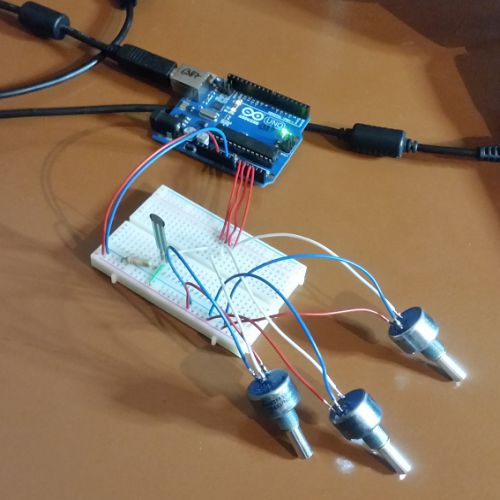
\includegraphics[scale=0.6]{image/Arduino_v0.jpg}
\end{center}
\caption{3 potentiomètres et une résistance de force connectés à un Arduino Uno.}
\label{fig:arduino_v0}
\end{figure}

En parallèle du développement logiciel, nous avons recherché une alternative aux FSR pour connaître la force sous les pieds de la chaise. 

Nous avons appris qu'il existe des capteurs appelés \textit{cellule de charge} permettant de mesurer très précisément une force. En effet, les cellules de charges sont des capteurs utilisés dans les pèses-personnes électroniques et des balances électroniques. Certains sont tellement précis qu'ils sont utilisés en laboratoire pour mesurer les quantités de produits chimique avec une précision de l'ordre du milligramme.

Nous allons vous expliquer comment ils fonctionnent et comment nous les avons utilisé pour se projet.

Le fonctionnement d'une cellule de charge se base sur la capacité qu'ont les conducteurs électriques à voir leur résistance changer lorsqu'ils sont déformés. Les conducteurs réalisant cette fonction s'appellent des jauges de contrainte (ou \textit{strain gauge} en anglais). Le principe est d'utiliser un matériau déformable et de fixer une ou plusieurs jauge de contrainte sur celui-ci au niveau des zones de déformation. Ainsi les jauges de contraintes vont suivre la déformation du matériau et changer de résistance. La figure \ref{fig:load_cell_sparkfun} illustre ces propos en montrant comment on la déformation d'un morceau de métal déforme aussi les jauges de contraintes (petit morceau de fil conducteur en zig-zag).

\begin{figure}
\begin{center}
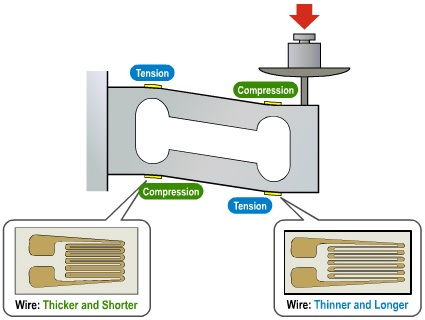
\includegraphics[scale=1]{image/load_cell.jpg}
\end{center}
\caption{Schéma d'une cellule de charge avec jauge de contrainte SOURCE: SPARKFUN.COM.}
\label{fig:load_cell_sparkfun}
\end{figure}

Au niveau des zones de compression la résistance est plus faible et au niveau des zone de tensions (ou d'étirement) elle est plus grande.

En effet, on a la formule de la résistance $R$ avec $\rho$ la résistivité du matériau conducteur, $l$ sa longueur et $S$ sa section: 

\begin{equation}
R= \rho \frac{l}{S}
\end{equation}

Si la jauge de contrainte est compressée, sa longueur $l$ diminue et sa section $S$ augmente. On a donc $R$ qui diminue.

Au contraire, si la jauge de contrainte est étirée, la longueur $l$ augmente et sa section $S$ diminue. On peut imagine un élastique qu'on étire, il s'amincit et s'allonge lorsqu'on l'étire.  On a donc $R$ qui augmente.

Seulement, vous l'aurez compris, les allongements et modifications de la section des jauges de contraintes sont très faibles si matériau sur lequel est construit la cellule de charge se déforme peu. Ces variations se produisent à une échelle du nanomètre et les variations de résistances résultantes sont donc de l'ordre du $m\Omega$ ou du $\mu\Omega$. Ce sont de ces capteurs que nous parlions au début de cette section du rapport.

Avec un Arduino, on ne peut pas mesurer les variations de résistances avec un simple montage diviseur de tension. Il est alors nécessaire d'introduire un montage appelé le pont de WheatStone permettant de transformer la mesure de la résistance en une mesure de tension (cf. figure \ref{fig:wheatstone_bridge}). Cependant, malgré le pouvoir amplificateur
du pont WheatStone, les variations de tensions sont trop faibles (de l'ordre du $mV$) pour être mesurés directement par l'Arduino. Il a donc été nécessaire en plus du pont de WheatStone d'utiliser un amplificateur pour cellule de charge.

\begin{figure}
\begin{center}
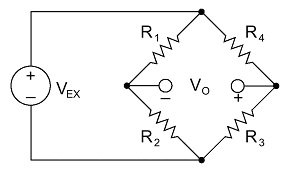
\includegraphics[scale=1]{image/wheatstone_bridge.jpg}
\end{center}
\caption{Schéma d'un pont de Wheatstone avec $V_{EX}$ la tension d'alimentation et $V_O$ la tension de sortie. SOURCE:NATIONAL INSTRUMENT}
\label{fig:wheatstone_bridge}
\end{figure}

Jérémy a réussi à récupérer les cellules de charges d'un pèse personne électronique. Ceux-ci sont connecté en demi pont de Wheatstone et utilisent seulement 2 jauges de contraintes. La figure \ref{fig:load_sensor} à quoi ressemble ces capteurs. Ceci veut dire que ces capteurs fournissent seulement les résistance $R_1$ et $R_2$ dans la figure \ref{fig:wheatstone_bridge}. Sur ces capteurs, les valeurs  de $R_1$ et $R_2$ sont d'environ 1$k\Omega$.

\begin{figure}
\begin{center}
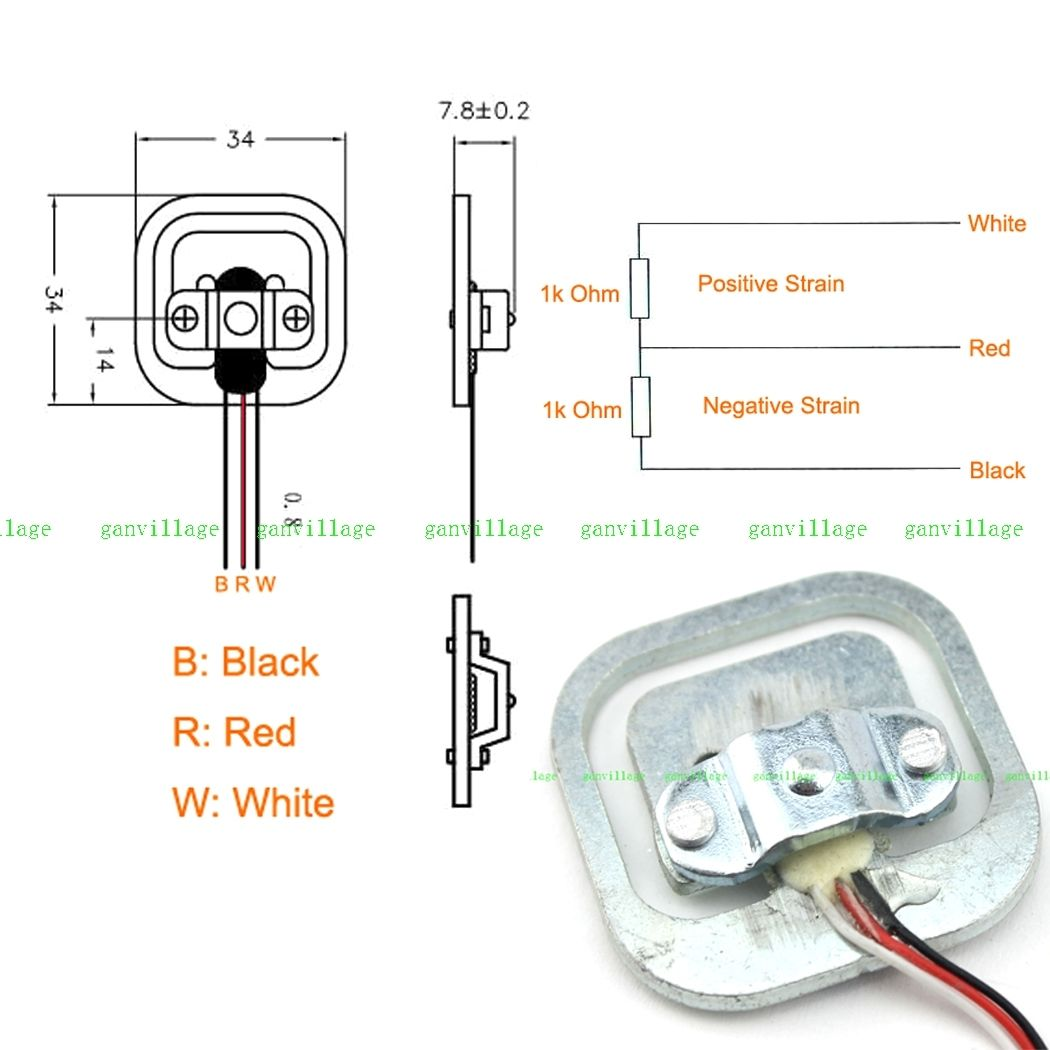
\includegraphics[width=12cm]{image/load_sensor.jpg}
\end{center}
\caption{Schéma d'une cellule de charge avec jauge de contrainte. SOURCE:ELECTRONIC STACK EXCHANGE}
\label{fig:load_sensor}
\end{figure}

Par la suite, le défi a été de réaliser 4 ponts de Wheatstone en couplant chaque cellules de charges à 2 résistances de 1$k\Omega$. Typiquement, on a placé 2 résistances fixes de $1k\Omega$ au niveau de $R_4$ et $R_3$.  On a pu ensuite connecter ces cellules de charges à des amplificateurs HX711 (cf. figure \ref{fig:load_sensor_connected}) pour obtenir un signal compatible avec l'Arduino.

\begin{figure}
\begin{center}
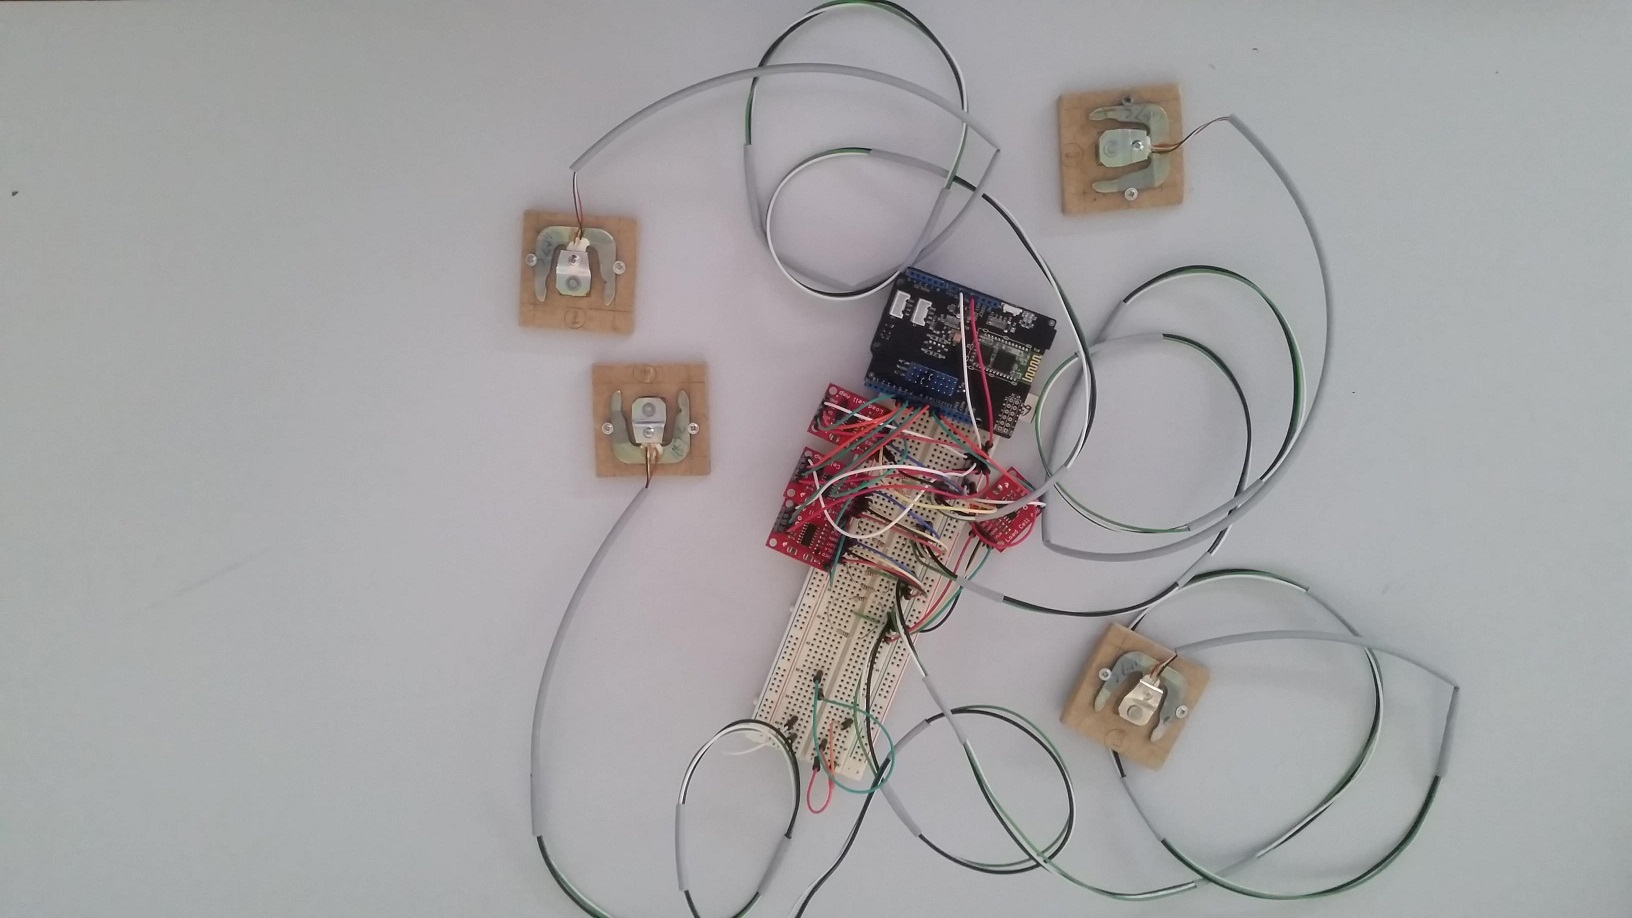
\includegraphics[width=12cm]{image/load_sensor_connected.jpg}
\end{center}
\caption{4 cellules de charges en demi-pont connectées à l'Arduino en utilisant des amplis HX711.}
\label{fig:load_sensor_connected}
\end{figure}

 En effet, les amplificateurs prennent un pont de wheatstone en entrée. On a donc connecté nos ponts de Wheatstone complet a l'amplificateur HX711 et connecté les amplis à l'Arduino au niveau des pins digitales. Les HX711 fournissent $V_{EX}$ et analysent $V_O$. L'amplificateur va d'une part amplifier le signal (la tension $V_O$) du pont mais aussi le convertir en signal numérique (digital) directement lisible par l'Arduino. Lors de la programmation de l'Arduino, nous avons donc utilisé une librairie permettant de contrôler et analyser les données de l'amplificateur HX711.
 
 Dans un optique de respect de l'environnement et de développement durable, nous avons cherché à estimer la consommation énergétique de notre prototype. Nous allons voir dans la prochaine section qu'il est possible d'alimenter notre prototype à l'aide d'une batterie portable servant à recharger un smartphone et ce pendant plusieurs heures.

\subsection{Consommation énergétique, autonomie et budget}

Nous avons cherché à déterminer la consommation énergétique et le prix de notre prototype.
L'idée derrière notre estimation et de faire la somme des consommations énergétiques de chaque éléments du prototype pour estimer la consommation totale.

En cherchant dans les documentations techniques des composants, nous avons pu établir un tableau de consommation pour chaque éléments (cf. table \ref{tab:consommation}).

\begin{table}
\begin{center}
\begin{tabular}{| c | c |}
\hline
\textbf{Matériau} & \textbf{Consommation} \\\hline\hline
Arduino & 50 mA \\\hline
Shield Bluetooth & 30 mA \\\hline
$4 \times$HX711 + Cellules de charge & 25 mA \\\hline
\textbf{Total} &  \textbf{105 mA} \\\hline
\end{tabular}
\end{center}
\caption{La consommation de chaque partie du montage électronique}
\label{tab:consommation}
\end{table}

Ces consommations sont les consommation moyennes observés pour chaque éléments pris uns par uns dans des conditions d'opération similaire aux notre. 
Nous avons cherché à comparer ces valeurs avec les valeurs réelles de notre circuit.

En connectant un ampèremètre en série avec les différents fils d'alimentations des composants électroniques, nous avons déterminé la consommation pratique de notre prototype.

\begin{figure}[htbp]
\begin{center}
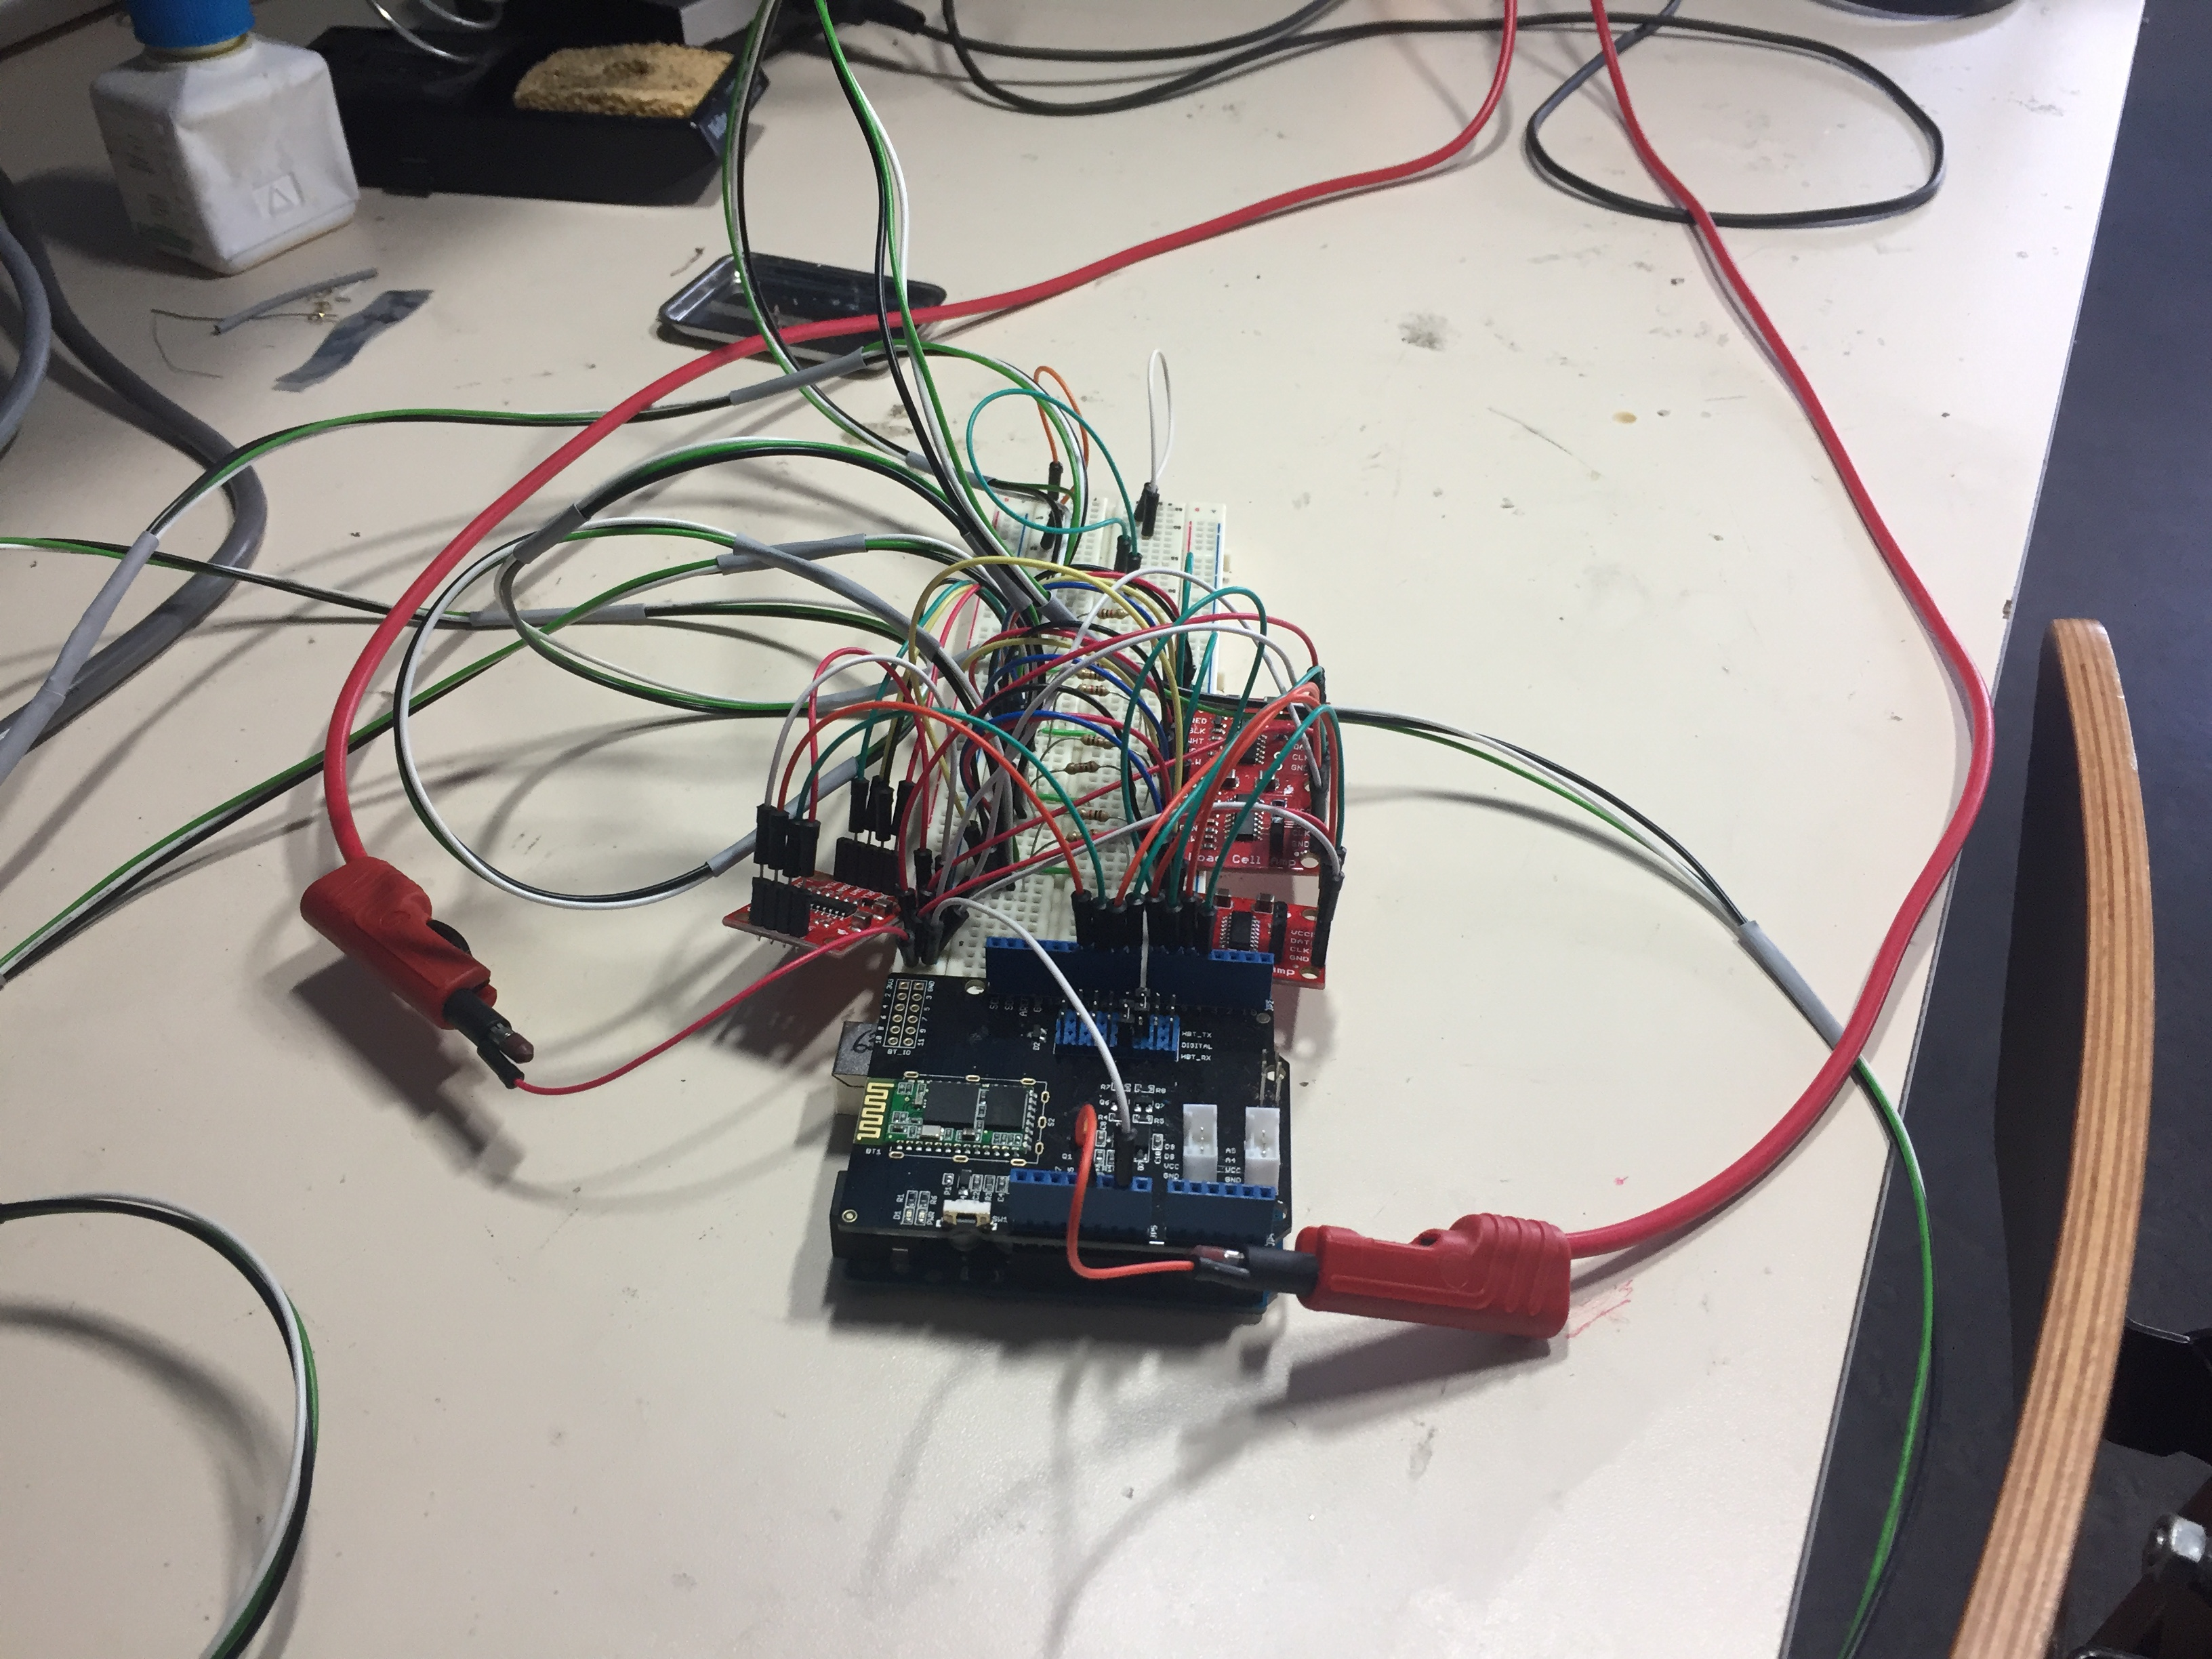
\includegraphics[width=12cm]{image/mesure_de_consommation1}
\end{center}
\caption{Mesure de la consommation de courant des amplificateurs HX711 connectés aux cellules de charges}
\label{fig:mesure_amper_hx711}
\end{figure}

La partie d'alimentation des amplificateurs HX711 connectés aux ponts de wheatstone (cf. figure \ref{fig:mesure_amper_hx711}) consomme environ 26mA à 5V c'est à dire une puissance d'environ 130mW.

En mesurant ensuite le courant consommé par l'ensemble Arduino + amplificateurs et cellules de charges (cf. figure \ref{fig:mesure_amper_tot}), nous sommes arrivés à une valeur moyenne de consommation de 113 mA à 5V c'est à dire une puissance de 0.566mW.

\begin{figure}[htbp]
\begin{center}
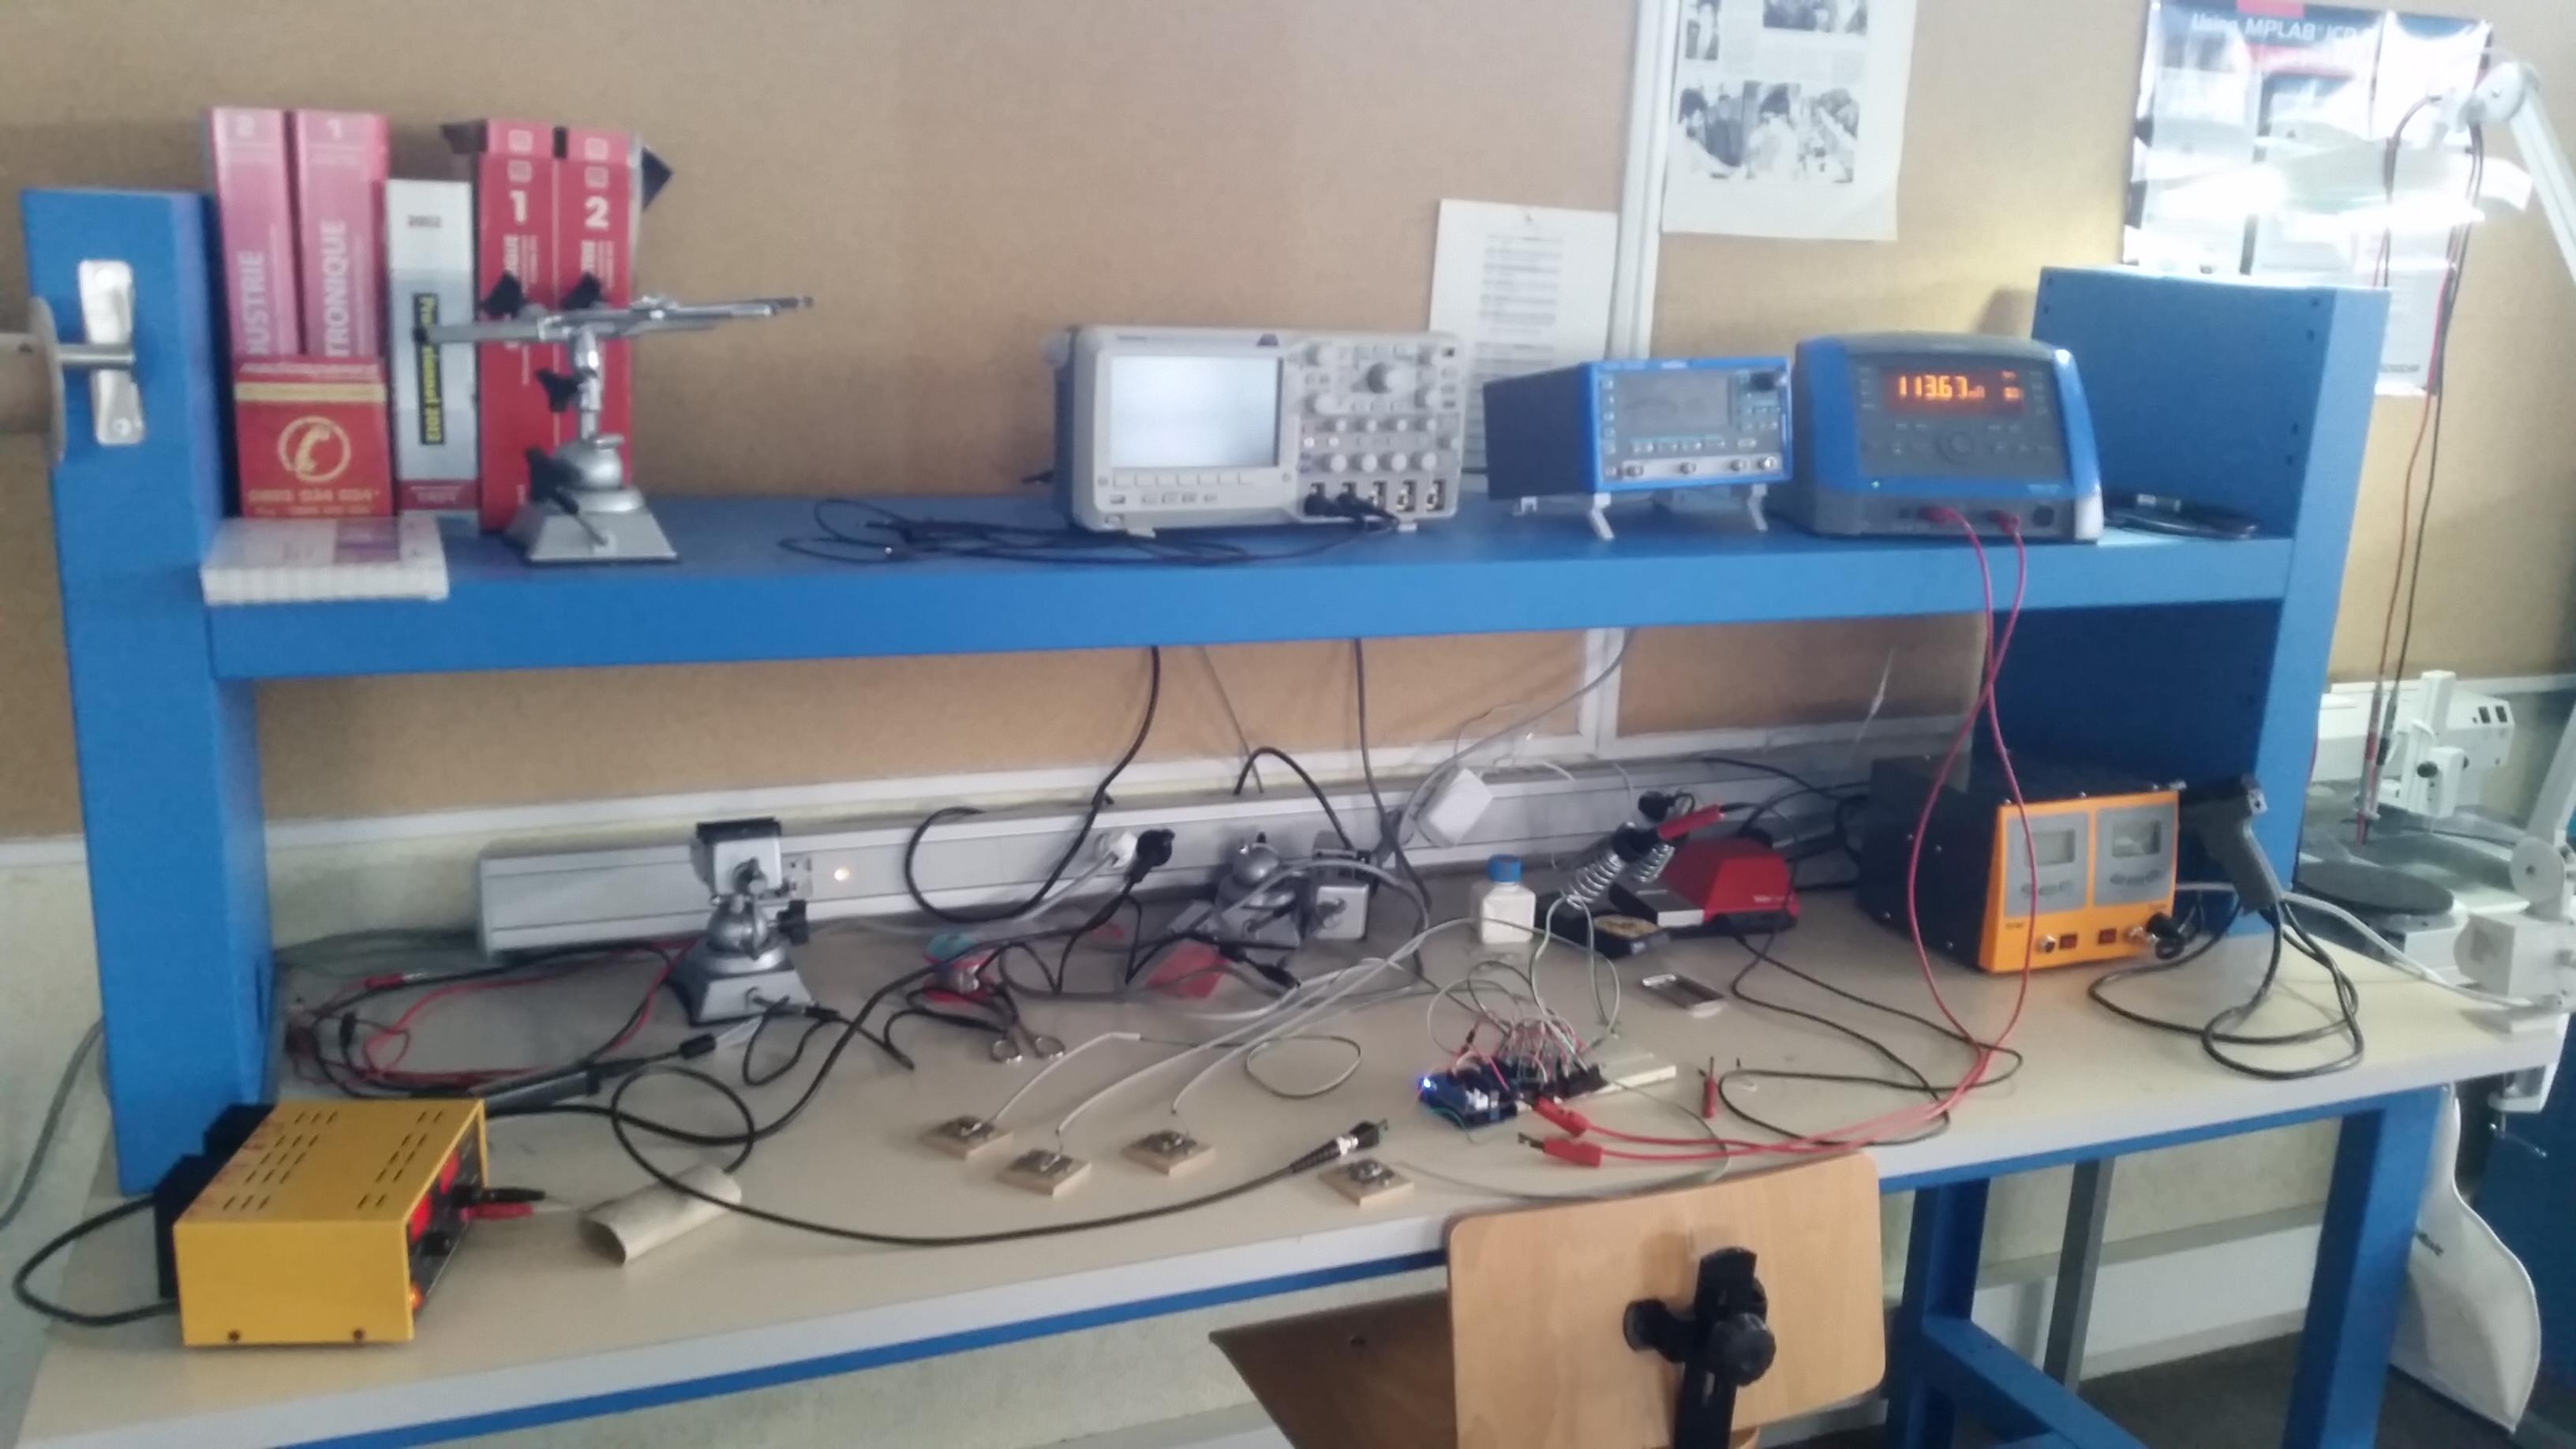
\includegraphics[width=12cm]{image/mesure_de_consommation2}
\end{center}
\caption{Mesure de la consommation énergétique totale du prototype}
\label{fig:mesure_amper_tot}
\end{figure}

On peut comparer cette consommation à celle d'une souris optique d'ordinateur.

En alimentant notre prototype à l'aide d'une batterie externe d'une capacité de 2000mAh, on va pouvoir faire fonctionner le prototype pendant une durée de d'environ 17h30 avant de devoir recharger la batterie (cf. equation \eqref{eqn:duree_fonct}).

\begin{equation}
\label{eqn:duree_fonct}
\text{Durée fonctionnement}
=
\frac{\text{Capacité}}
{\text{Consommation de courant}}
= \frac{2000\text{mAh}}{113\text{mA}}
=17.69 h
\end{equation}


On pourrait réduire cette consommation énergétique en utilisant un modèle d'Arduino plus petit tel que l'Arduino Pro Mini. 
On peut aussi éteindre les LEDs de l'Arduino pour réduire la consommation de quelques dizaines de mA.
De même on aurait pu avec plus de temps rajouter un boutons poussoir permettant de mettre en veille l'Arduino et les amplificateurs si personne n'est assis sur la chaise.

Nous avons aussi étudié la dimension économique du prototype. 
Nous avons ensuite estimé le prix de reviens de notre prototype (cf. table \ref{tab:prix_amazon}). 

\begin{table}
\begin{center}
\begin{tabular}{| c | c |}
\hline
\textbf{Matériau} & \textbf{Prix} \\\hline\hline
Arduino & 20 € \\\hline
Shield Bluetooth & 25 € \\\hline
$4 \times$HX711 & 1,80 € (par pièce) \\\hline
$4 \times$Cellule de charge & 12 € \\\hline
Batterie Lithium externe pour smartphone (2000 mAh) & 10 € \\\hline
Cable USB-B$\rightarrow$A & 2 € \\\hline
Breadbord (plaque prototype) \& Fils de connexion & 9 € \\\hline
$8 \times$Résistance (1 k$\Omega$) & 0,04 € (par pièce) \\\hline
\textbf{Total} &  \textbf{85,52 €} \\\hline
\end{tabular}
\end{center}
\caption{Le prix de chaque partie du montage électronique sur \textit{Amazon}}
\label{tab:prix_amazon}
\end{table}


Il est possible de diminuer le cout de ce prototype en remplaçant l'Arduino Uno par un modèle Arduino Pro mini en moyenne 50\% moins cher que la version Uno. De même on peut remplacer le Shield Bluetooth par un module Bluetooth HC-05 coutant environ 5€ contre 25€ pour le shield.
Nous avons tout de même fait attention aux cout de ce prototype en choisissant des cellules de charges de pèse personne électronique au lieu de cellules de charge plus performante.
 En effet, celle-ci atteignent des coût proche de 100 € pièce contre 4€ pièce pour les cellules que nous avons récupéré.

\textbf{Transition:} Nous avons désormais fait le tour du matériel que nous avons étudié et utilisé pour réaliser ce projet. Nous allons maintenant nous intéresser à l'aspect logiciel de ce projet qui consiste d'une part à programmer l'Arduino pour qu'il lise les valeurs des capteurs de forces et d'autre part à communiquer avec une interface utilisateur (un Smartphone ou un PC) pour donner les résultats et l'interprétation à l'utilisateur.


\chapter{Le développement du logiciel}
\label{chap:logiciel}

En parallèle de la conception de l'électronique du correcteur de posture, nous avons travailler sur un programme de visualisation de la posture de l'utilisateur. Nous avons beaucoup travaillé avec la version \ref{fig:arduino_v0} pour développer le logiciel de l'Arduino et l'interface graphique sur PC et Android. Lorsque la commande des amplificateurs HX711 et des cellules de charges est arrivé, nous avons simplement modifié très légèrement le logiciel de l'Arduino pour qu'il utilise les amplificateurs au lieu des potentiomètres de la version \ref{fig:arduino_v0}. Le fonctionnement général des 2 versions (potentiomètres et amplis) est similaire et ne diffère que dans la façon d'initialiser les capteurs et récupérer la valeur des capteurs. Les données récupéré seront identiques et l'interprétation donnée par les deux versions est la même.

Commençons donc par la programmation de l'Arduino et la gestion des capteurs.

%Une fois que la partie électronique du correcteur de posture est réalisée, et que donc les capteurs fournissent une tension mesurable à l'Arduino, il est temps de passer au développement du logiciel qui va nous permettre de visualiser la posture de l'utilisateur. Ce développement commence, évidemment, au niveau de l'Arduino.

\section{Bas niveau : l'Arduino}
\label{sec:logiciel_bas}

Le langage de programmation utilisé pour programmer l'Arduino est peu différent de C ou C++; en fait, il est basé sur ces langages. Le code, après quelques petits changements, est compilé par un compilateur \texttt{avr-g++} (compilateur C/C++). Pour le programme de l'Arduino, nous avons choisi d'utiliser surtout la syntaxe C ; nous avons toutefois utilisé aussi quelques fonctions C++ pour rendre notre programme plus efficace. Nous avons donc utilisé l'EDI Arduino (Environnement de développement informatique) officiel disponible à l'adresse \url{https://www.arduino.cc/} gratuitement. Cet environnement nous a permis d'écrire du code C et C++ et de le télé-verser dans la mémoire de l'Arduino. Il possède aussi des fonctions intéressantes tels qu'un moniteur série permettant d'avoir un endroit où on peut afficher des messages envoyés par l'Arduino.

Le but du programme de l'Arduino est de récupérer les données que fournissent les amplificateurs à partir des cellules de charge, de les traiter afin de n'avoir que des valeurs valides, et enfin de les envoyer (que ce soit par USB ou par Bluetooth) à l'application (que ce soit l'application PC ou celle d'Android).

En travaillant avec la version utilisant des potentiomètres, on pouvait récupérer les valeurs des potentiomètres en éxecutant la commande \texttt{AnalogRead(A\#)} avec \textbf{\#} le numéro du pin Analog sur lequel on a connecté le potentiomètre. On se rappelle que l'entrée au niveau du pin Analog est un montage diviseur de tension. Ce montage fournis comme on l'a vu dans le chapitre précédent \ref{chap:arduino} une tension entre 0 et 5V au niveau du pin Analog. La commande  \texttt{AnalogRead(A\#)} permet de convertir cette valeur de tension en un nombre entier compris entre 0 et 1023 (donc 1024 valeurs possibles).

Dans la version utilisant les amplificateurs, on a utilisé la librairie HX711 (\url{https://github.com/bogde/HX711}) permettant de récupérer les valeurs des capteurs sur les pins digitals de l'Arduino. 
Cette fois on récupère le nombre entier à l'aide de la commande \texttt{sensor.get\_unit()} ou \texttt{sensor.get\_value()} (\texttt{sensor} est l'objet représentant l'ampli dans le code C). 
Sans calibration de l'amplificateur, ce nombre est brut et n'a pas de sens. 
On applique alors des corrections notamment en faisant le zéro des amplificateurs avec la commande \texttt{sensor.tare()}.
 \'A ce moment, la valeur retournée par l'amplificateur augmentent de manière linéaire avec la force appliqué au capteur (elle a donc du sens).

\'Etant donné qu'on a fabriqué des demi-ponts de Wheatstone, ils sont sensibles aux variations de températures et la valeur des capteurs peut fluctuer. 
La valeur donnée par les amplificateurs a donc tendance à fluctuer (les fluctuations sont de l'ordre de \textpm 5) et peut parfois prendre des valeurs négatives par rapport au zéro obtenu par la tare.
 Pour essayer de compenser ce problème, premièrement, on a pris la valeur absolue des valeurs (on supprime alors les fluctuations négatives). 
En effet, l'idée derrière cette correction est que lorsque le capteur ne peux avoir que des valeurs positives ou nulles.
 La valeur nulle est la valeur au repos et la valeur augmentera lorsque une force sera appliqué sur le capteur.
  Un deuxième correction a été d'ajouter un décalage (offset) des valeurs obtenus pour faire en sorte de ne jamais avoir 0. 
  Comme on a montré avec la formule \eqref{eq:centre_gravite_vectorielle}, si les valeurs des capteurs sont toutes nulles en même temps, la position du centre de gravité sera $(0, 0)$. 
  Or on a voulu que, lorsque les capteurs sont au repos (donc après une tare), le centre de gravité coïncide avec le centre de la chaise.
   Pour cela, il faut impérativement que peut importe la géométrie de la chaise, les valeurs au niveau des capteurs soient non nulles.


% D'abord, donc, on récupère les données en faisant un \textit{read} sur les capteurs; on enregistre ces valeurs à un tableau de quatre entiers (\texttt{int}), après avoir pris leur valeur absolue, et avoir fait un \textit{offset}. Ceci est nécessaire, car les petites variations de température entre les cellules de charge donnent naissance à des variations de tension, qui sont ensuite amplifiées. Pour corriger ce paramètre, il est nécessaire de prendre la valeur absolue des données fournies par les capteurs de charge (en réalité, il est impossible qu'une personne applique une force négative aux capteurs !). Ensuite, pour vérifier que la valeur minimale des capteurs ne sera jamais 0 pour tous les capteurs, on prend soin de décaler les valeurs obtenues; comme on a montré avec la formule \ref{eq:centre_gravite_vectorielle}, si les \guillemotleft ~masses~\guillemotright\ des capteurs sont tous nuls en même temps, la position du centre de gravité sera $(0, 0)$. Au cas où aucune charge n'est appliquée aux capteurs, le centre de gravité doit coïncider avec le centre de la chaise.

Une fois ce travail achevé, on envoie les données à l'application. On sera en mode série, ce qui implique qu'on enverra les données octet par octet. Il est évident que cette option sert à mettre à jour les données en temps réel, en assurant en même temps une faible éventualité de pertes d'information ou de données incomplètes.
%, étant donné qu’on envoie un seul octet à la fois.
Un périphérique utilisant une liaison série possède voies de communication. La première est la voie RX permettant de recevoir les données (octets). La seconde est la voie TX permettant de transmettre les données.  Si on veux faire dialoguer deux périphérique série, il faut connecter la voie TX et RX de l'un respectivement sur les voies RX et TX de l'autre.

\begin{eqnarray}
TX_1 \rightarrow RX_2
\\
RX_1 \leftarrow TX_2
\end{eqnarray}

Ainsi les données envoyées par l'un sont reçu par l'autre et vis-versa. Ce mode de connexion est dit \guillemotleft croisé \guillemotright .
Cependant pour que deux périphériques séries communiquent entre-eux, il faut qu'ils parlent le même langage c'est à dire que les paramètres de communication soient les même.

On commence donc en initialisant la communication série, ce qui veut dire qu'on doit choisir les paramètres de communication. Afin d'obéir aux standards de l'Arduino, nous avons fixé les paramètres de communication de la façon suivante :

\begin{itemize}
\item \textit{BaudRate} (vitesse de communication) : 9600 bauds
\item \textit{DataBits} (nombre de bits de données) : 8
\item \textit{StopBits} (nombre de bits de stop) : 1
\item \textit{Parity} (parité du message) : NO\_PARITY (pas de parité)
\end{itemize}

Pour tous ces paramètres, hormis le premier, nous avons choisi de suivre les standards mis en place par l'Arduino : 8 bits de données, 1 bit de stop, et pas de parité de message.
Tout les périphériques séries utilisés pour communiquer ( l'Arduino, le PC, le smartphone Android, le module bluetooth) sont configurés de cette façon de manière à ce que tous se comprennent.
 %Pour la communication, nous avons choisi un \texttt{baud rate} de 9600, car nous voulons que la communication se passe rapidement, mais pas au point de nous donner des résultats incohérents, dans le cas où sont impliqués des appareils ou des ordinateurs différents. En choisissant 9600 bauds, on obtient une vitesse confortable et une bonne compatibilité tant en Bluetooth qu'en USB.

Pour transmettre les données on a utilisé le port USB B intégré à l'Arduino. La connexion est donc directe entre le PC et l'Arduino. Le PC reconnais alors l'Arduino en tant que périphérique de communication série et on peut dialoguer sans problème. On a donc le schéma suivant pour la communication USB.

\begin{eqnarray}
TX_{Arduino-USB} \rightarrow RX_{PC}  \\
RX_{Arduino-USB}  \leftarrow TX_{PC}
\end{eqnarray}

Pour effectuer une liaison série en Bluetooth, on a utilisé un shield Bluetooth car l'Arduino ne possède pas de module bluetooth installé en usine. Le shield bluetooth un circuit électronique comprenant un module bluetooth conçu pour l'Arduino et venant se connecté sur celui-ci. En fait, le module bluetooth communique avec l'Arduino via le protocole série et le module bluetooth communique en série avec la carte bluetooth du PC ou du smartphone. On a donc le schéma suivant pour la communication Bluetooth.

\begin{eqnarray}
TX_{Arduino-Digital} \rightarrow RX_{Shield-Digital} \rightarrow TX_{Shield-Bluetooth} \rightarrow RX_{PC/Smartphone}  \\
RX_{Arduino-Digital} \leftarrow TX_{Shield-Digital} \leftarrow RX_{Shield-Bluetooth} \leftarrow TX_{PC/Smartphone}
\end{eqnarray}

On a donc utilisé deux pins digital de l'Arduino pour communiquer en série avec le Shield. 
Ainsi l'Arduino est connecté physiquement au module bluetooth et le module bluetooth est connecté sans fil au PC ou smartphone. 
On voit bien avec ce schéma que le shield bluetooth est un intermédiaire. 
Les données envoyés par l'arduino (sur la voie TX du port digital) se retrouvent bien sur la voie TX du bluetooth.
 De même les données arrivant sur la voie RX du bluetooth se retrouvent bien sur la voie RX de l'Arduino.
  Il a fallu suivre ce diagramme lors de la programmation et de la configuration des différents pins utilisés pour la communication série car on peut rapidement se tromper.

Une fois qu'on a initialisé la communication, on peut envoyer les données. Nous rappelons que le but est d’envoyer les 4 différentes valeurs obtenues à partir des 4 capteurs. Avant même de discuter le processus de l'envoi des données des capteurs, on sait qu'on doit envoyer un caractère qui \textit{initialise} le message, ainsi qu’un autre qui le \textit{termine}. Ceci sert à distinguer les messages entre eux, et à vérifier que toutes les données sont bien transmises. Pour initialiser le message, on envoie un caractère ASCII \guillemotleft ~STX \guillemotright\ (start of text), qui a pour code le nombre décimal 2. Pour terminer le message, on envoie un caractère \guillemotleft\ CR~\guillemotright\ (enter/carriage return), qui a pour code le nombre décimal 13. Notre module de communication sur l'application (qu'elle soit en PC ou en téléphone portable) est avertie désormais que les données des capteurs seront comprises entre ces deux caractères.

%Pour l'envoi des données des capteurs, nous avons décidé que le meilleur message serait court et simple.
%Ainsi, on diminue encore plus le danger de transmettre ou de recevoir des données incomplètes, car on envoie le minimum absolu des caractères. FAUX ne pas mettre
Comme on ne connaît pas la taille de la valeur de chaque capteur (c'est-à-dire le nombre des chiffres), on ne peut pas les envoyer directement l'un après l'autre, il nous faut donc un séparateur.
Nous avons choisi un caractère point-virgule (\guillemotleft ; \guillemotright), car il offre une séparation visuelle mais aussi sémantique. Toutefois, pour cette application n'importe quel caractère pourrait être choisi comme séparateur tant que ce n'est pas un chiffre ou un caractère délimiteur (STX ou CR). Le format de chaque message est donc le suivant :

\begin{center}
\texttt{STX (02)}\\
\texttt{valeur1;valeur2;valeur3;valeur4}\\
\texttt{CR (13)}
\end{center}

%où \texttt{02} et \texttt{13} sont les caractères \texttt{STX} et \texttt{CR} respectivement, et \texttt{valeur1, valeur2, valeur3, valeur4} sont les nombres entiers obtenues à partir des 4 capteurs. 
où \texttt{valeur1, valeur2, valeur3, valeur4} sont des chaines de caractères ASCII représentant les nombre entiers/valeurs des capteurs. 
%Comme on l'a dit plus haut, les valeurs sont transmises caractère par caractère, et non pas toutes en même temps.

%Finalement, afin d'éviter d'envoyer des données qui ne changent pas (ou alors qui changent très peu), nous avons mis en place un petit \guillemotleft timer \guillemotright , qui fait qu'on envoie des données tous les 100 millisecondes.
Finalement, nous avons décidé d'envoyer ces données toutes les 100 millisecondes pour avoir une mesure réactive de la posture. Il a donc fallu implémenter un pause c'est à dire un \guillemotleft timer \guillemotright  dans l'envoie des données.
 Une implémentation de premier niveau consisterait à arrêter le programme pour 100 millisecondes avant d'envoyer à nouveau des données, mais elle n'est pas tout a fait correcte.
  Si, pendant le temps d'arrêt, on veut avoir accès aux données, ou par exemple envoyer des commandes à l'Arduino à partir de l'application PC ou Android, il risque d'y avoir des problèmes, car le programme sera en pause pendant ce temps-là.
   Pour éviter ce problème, nous avons implémenté la fonctionnalité de manière \textit{asynchrone} : on calcule la différence entre le temps dit \guillemotleft du début \guillemotright\ et le temps dit \guillemotleft actuel \guillemotright . 
   Si cette différence est supérieur ou égale à 100 millisecondes, on lit les données à partir des capteurs et on les envoie, puis on met à jour le temps dit \guillemotleft du début \guillemotright . 
   Cela nous permet d'avoir accès aux autres fonctionnalités de l'Arduino, en limitant en même temps les données envoyés.


\textbf{Transition:} Nous avons pu voir comment nous avons choisis de récupérer les données des capteurs et les transmettre à l'ordinateur ou le smartphone qui va se charger de la visualisation. Intéressons-nous sans attendre aux programmes PC et Android que nous avons conçu pour permettre à l'utilisateur de visualiser sa posture.

\section{Haut niveau : les applications PC et Android}
\label{sec:logiciel_haut}

%Pour gérer les données fournies par les load sensors, nous devons construire une application qui visualise la posture assise de l'utilisateur. 
Pour interpréter les données fournies par les capteurs de charges, nous avons du concevoir une application permettant de visualiser la posture assise de l'utilisateur.
 Cette partie aura pour but de vous présenter notre solution logicielle dont nous aborderons quelques détails de réalisation par la suite.
Pour le développement de cette application, nous avons choisi \texttt{Java} comme langage de programmation. Il est conforme avec cette tâche, et il nous est accessible à travers notre cursus académique. En réalité, nous l'avions déjà utilisé, aussi bien pour les projets PeiP de la première année, que pour des projets personnels.

Pour mieux organiser notre travail et afin d'avoir accès aux versions précédentes de notre logiciel, nous avons utilisé \texttt{git} comme \textit{VCS} (logiciel de contrôle des versions). Suite à la création d'un dépôt sur \texttt{GitHub}, nous avons pu synchroniser nos fichiers locaux, gérés par \texttt{git}, sur le dépôt en ligne. Cela nous a permis de mettre en jour le projet, et mettre en communs les changements effectués facilement.

Pour que notre application soit polyvalente, nous avons décidé de mettre en place une version PC et Android (voir figures \ref{fig:screenshot_pc} et \ref{fig:screenshot_android}). De cette manière, l'utilisateur peut consulter le correcteur de posture depuis son ordinateur ou son téléphone portable.

\begin{figure}[htbp]
\begin{center}
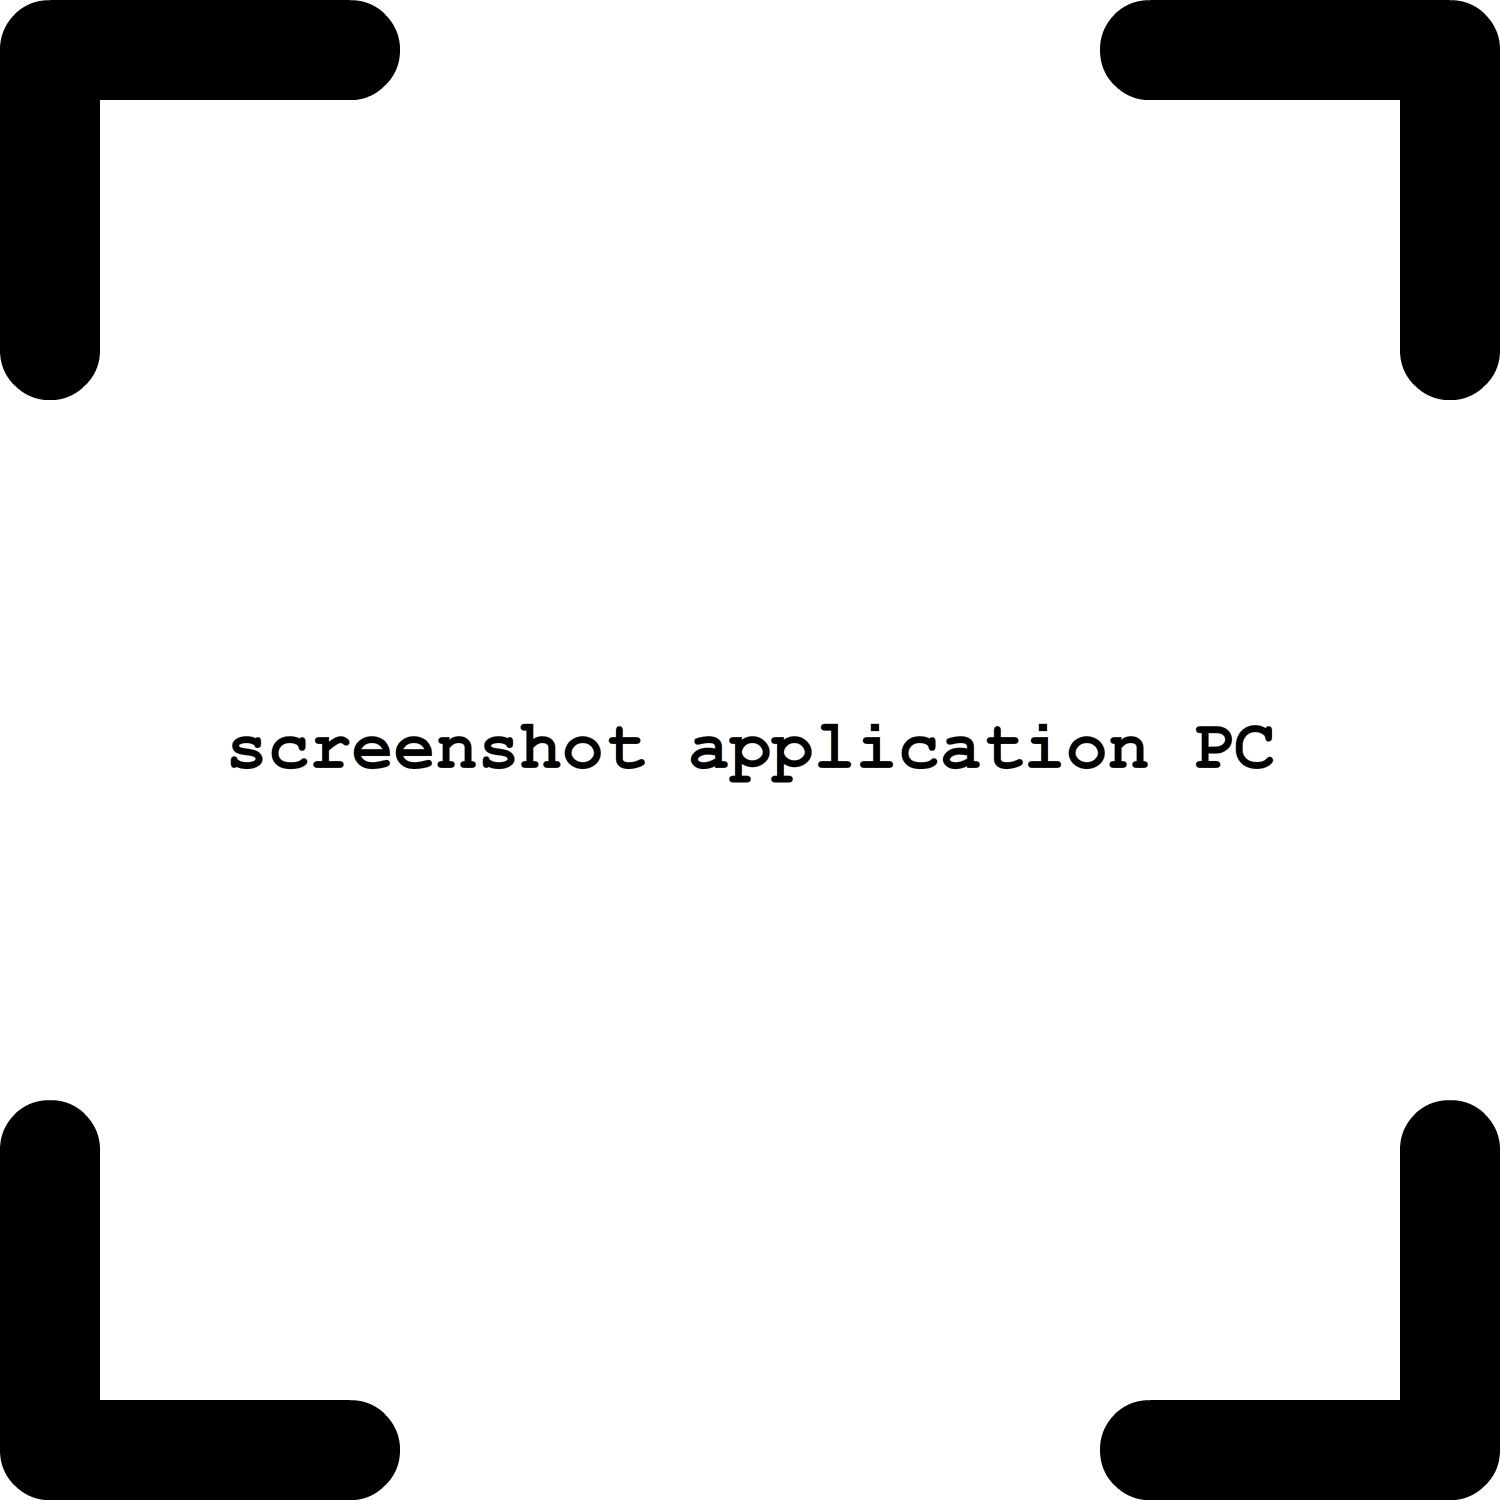
\includegraphics[width=12cm]{image/screenshot_pc1}
\end{center}
\caption{L'application PC.}
\label{fig:screenshot_pc}
\end{figure}

\begin{figure}[htbp]
\begin{center}
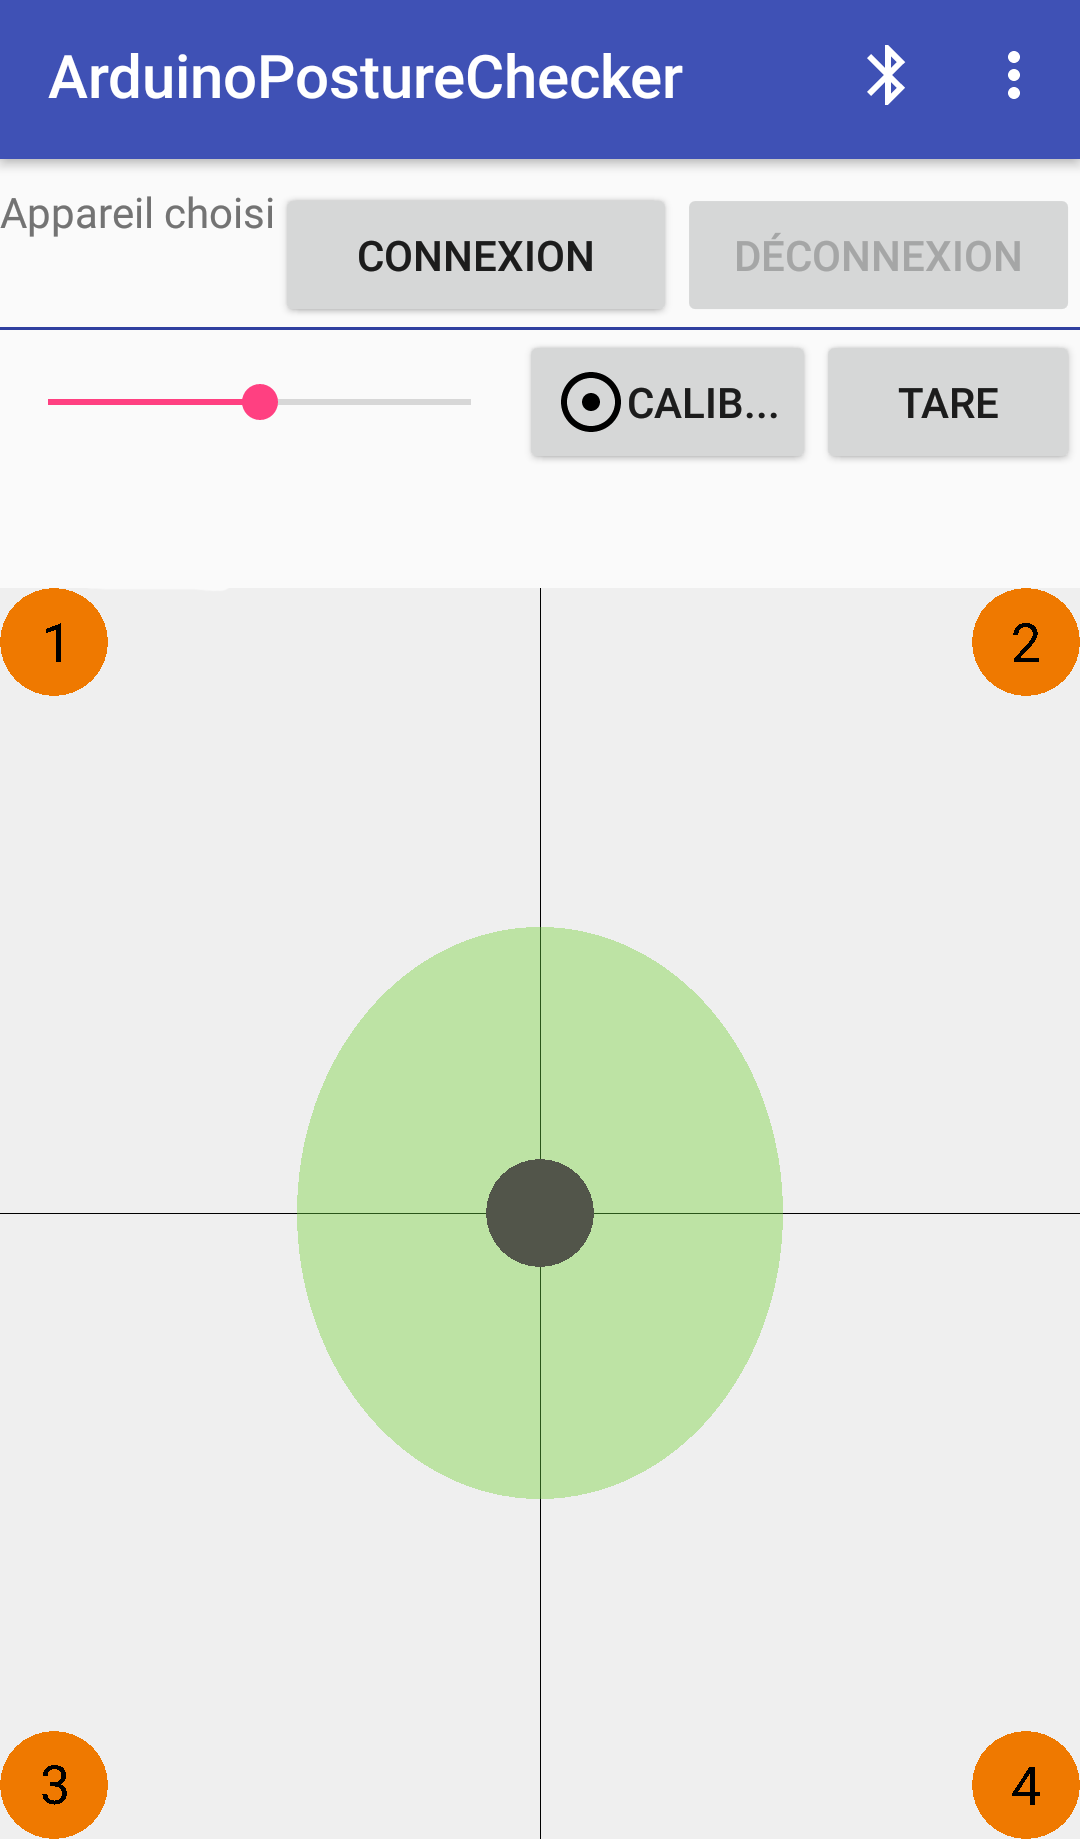
\includegraphics[width=12cm]{image/screenshot_android1}
\end{center}
\caption{L'application Android.}
\label{fig:screenshot_android}
\end{figure}

Le design général de l'application dans les deux cas reste le même, indépendamment de la plateforme :  une partie est dédiée à la visualisation de la chaise, et l'autre est dédiée à la configuration (qu'elle concerne la chaise, la visualisation où la communication bluetooth). 

Dans la partie visualisation, on a représenté les pieds de la chaise par des cercles auxquels s'associe un nombre, correspondant à l'ID de chaque capteurs. Pour une chaise banale à quatre pieds, on aura donc quatre cercles, situés aux quatre coins de la zone de visualisation, et portant des nombres 1, 2, 3 et 4.
Cette zone de la visualisation comprend en outre le centre de gravité de la personne assise, qui est donné par la formule \eqref{eq:centre_gravite_vectorielle}. Le centre de gravité est représenté par un cercle noir, qui se déplace dans en suivant les changements de la posture de l'utilisateur.

Finalement, nous avons aussi inséré la \guillemotleft  deadzone\footnote{La deadzone est le nom qu'on donne à la zone de confort, c'est à dire la zone où on considère l'assise correcte.} \guillemotright, c'est-à-dire la zone dans laquelle la posture assise est considérée idéale. Traduit littéralement, ce mot signifie la zone morte. C'est un nom qu'on donne à un périmètre délimitant une zone où il est sensé ne rien se passer. Ici, si le centre de gravité est dans la zone, on est bien assis alors il ne se passe rien. Elle est représentée par un cercle vert, dont on peut modifier la taille ainsi que la position. Cela garantit que si on a une chaise différente (par exemple une chaise à trois ou à cinq pieds), l'utilisateur peut déplacer la position de la deadzone selon ses besoins : il suffit de prendre la posture considérée comme idéale, puis de calibrer la deadzone en cliquant sur le bouton correspondant.

En somme, notre solution permet les manipulations suivantes :
\begin{itemize}
\item Modifier le nombre et les positions des pieds de la chaise;
\item Modifier la position et la taille de la deadzone;
\item Sauvegarder la chaise;
\item Utiliser une chaise déjà enregistrée.
\end{itemize}


Pour utiliser l'application, il faut d'abord configurer la chaise. On clique sur le bouton \guillemotleft ~configuration~\guillemotright\ , on saisit le nombre des pieds de la chaise et leurs positions (on supposera que pour une chaise à quatre pieds, le pied qui se trouve devant et à gauche est au point (0,0). Les positions des autres pieds seront mesurées relativement au point (0,0) qu'on a défini).
 Une fois que la chaise est configurée, on peut se connecter à l'Arduino, soit par Bluetooth (auquel cas il faut appairer le smartphone ou PC au shield Bluetooth de l'Arduino au préalable afin de pouvoir s'y connecter), ce qui est préférable, soit par USB. 
Finalement, on doit s'asseoir correctement, afin de calibrer l'application.
Pour ce faire, il faut ,avant de s'asseoir sur la chaise, appuyer sur le bouton \guillemotleft ~tare \guillemotright . Cette action fera le zéro des capteurs et le centre de gravité se retrouvera déplacé au centre de la zone de visualisation. On peut ensuite s'asseoir dans la position désiré puis appuyer sur le bouton \guillemotleft\ calibrer~\guillemotright . Une fois la calibration terminée, la deadzone est centrée sur la position du centre de gravité désirée. Finalement on peut modifier sa taille selon nos préférences. 

Maintenant, l'application affichera la deadzone et le barycentre, qui deviendra rouge quand il sort de la deadzone, ce qui veut dire que notre posture n'est pas bonne.
 En ce point, on peut sauvegarder la chaise afin d'éviter la procédure de configuration chaque fois qu'on veut utiliser l'application. 
Pour ce faire, on clique sur \guillemotleft ~sauvegarder chaise~\guillemotright\ , puis on choisit un dossier et un nom pour notre chaise (la chaise sera sauvegardée dans un fichier \texttt{.txt}). 
La prochaine fois qu'on ouvrira l'application, on pourra cliquer sur \guillemotleft ~charger une chaise~\guillemotright\  et donc charger le fichier qu'on a enregistré.
 Ce fonctionnement nous permet aussi d'utiliser plusieurs chaises sans avoir besoin de changer la configuration chaque fois qu'on utilise une chaise différente.

Bien que notre matériel soit conçu pour une chaise à quatre pieds banale, nous avons tout de même tenus à développer un logiciel aussi général et polyvalent que possible.
En effet, il peut fonctionner avec n'importe quel type de chaise avec n'importe quel nombre de pieds.

Pour arriver à ce résultat, nous sommes passés par plusieurs étapes. L'objectif de la suite du rapport sera de les détailler.

\subsection{La communication série}
\label{subsec:comm_serie}
La première chose sur laquelle nous avons commencé à travailler est un élément essentiel de notre application, tout comme la modélisation de la chaise décrite dans la sous-section \ref{subsec:model_chaise}. Il s'agit de la partie \textit{communication}. C'est grâce à ce module qu'on peut finalement recevoir les données des capteurs dans un contexte qui permet de les visualiser et de les rendre plus faciles à interpréter par l'utilisateur.

L'idée ici a été de trouver un moyen de manipuler les liaisons série de l'ordinateur pour permettre à l'Arduino de communiquer avec le PC où le smartphone.
Pour cela, on a utilisé la librairie JAVA open-source \texttt{jSerialComm} [REFERENCE BIBLIOGRAPHIQUE]. Nous avons ensuite utilisé le code que Jérémy avait écrit pendant son stage de PeiP1 pour communiquer avec les ports série de l'ordinateur. On a donc pu rapidement élaborer un module JAVA permettant de communiquer avec l'Arduino sur lequel nous avons greffé l'interface graphique. La librairie jSerialComm est très complète et permet de lister et configurer tout les ports séries disponibles sur l'ordinateur à notre guise. Nous avons donc utilisé le standard défini dans la section \ref{sec:logiciel_bas} lorsque nous parlions de l'Arduino à savoir:

%Ce module est basé sur la librairie \texttt{jSerialComm} [REFERENCE BIBLIOGRAPHIQUE]. Il obéit, comme nous avons dit, au protocole suivant :

\begin{itemize}
\item \textit{BaudRate} (vitesse de communication) : 9600
\item \textit{DataBits} (nombre de bits de données) : 8
\item \textit{StopBits} (nombre de bits de stop) : 1
\item \textit{Parity} (parité du message) : NO\_PARITY (pas de parité)
\end{itemize}

On peut ensuite utiliser les ports séries à travers des flux d'entrée et de sorties. Ils se présentent sous la forme d'objets standards de la classe \texttt{java.io}. On reçoit les données dans un objet \textit{InputStream} retourné par le port série sélectionné avec la librairie jSerialComm puis on envoi les données dans un objet \textit{OutputStream} retourné par le port série. Ainsi, comme on l'a vu précédemment, les octets transmis à l'ordinateur au niveau du port série via la voie RX arriveront dans l'objet \textit{InputStream} et les données sortantes de l'ordinateur via \textit{l'OutputStream} se feront sur la voie TX.

La librairie jSerialComm prends en charge la carte Bluetooth de l'ordinateur, si celui-ci en est équipé, et permet d'ouvrir des flux de communication série en Bluetooth de la même manière que pour un ports série physique. Le fonctionnement Bluetooth a donc été totalement transparent et implémenté d'office au niveau de l'application PC.

Concernant l'application mobile, nous avons utilisé une partie du code rédigé par Jérémy lors de son projet de PeiP1 qui utilisait aussi la communication bluetooth série sur Android.
 Le module bluetooth sur Android fonctionne grâce à l'API bluetooth   d'Android. 
Nous nous sommes basés sur l'exemple \textit{BluetoothChat} fourni par Google dans son EDI Android Studio. L'idée reste cependant la même, la programmation se fait en JAVA et la réception et l'émission de données se font à travers des objets java.io.InputStream et java.io.OutputStream. 
La communication pour le PC et Android est donc identique.

%Nous pouvons désormais communiquer avec l'Arduino, en imposant un protocole commun pour les deux appareils.
%Le module est capable de trouver tous les \textit{ports} de communication série disponibles sur l'ordinateur (ou le téléphone portable).
% On peut ensuite les lister et accorder à l'utilisateur le lancement d'un flux de communication à travers un de ces ports. Ce flux permet de recevoir et envoyer des données : nous rappelons que, même si la fonction principale de l'application est de recevoir des données à partir des senseurs et de les interpréter, on doit être capable d'envoyer une commande afin d'effectuer une \textit{tare}, et réinitialiser ainsi les senseurs.

Enfin, nous avons ajouté aux modules de communications un \guillemotleft ~parser~\guillemotright , c'est à dire une sorte de déchiffreur pour interpréter les données reçues au niveau des flux.
 Le parser analyse les octets et les organise dans un tableau d'entiers de façon que la valeur et l'ID des capteurs soient facilement récupérables pour être utilisés par la suite.
Cette fonctionnalité permet aussi de savoir si on a reçu des données incomplètes, ou même si on n'a rien reçu depuis l'Arduino. En effet, le parser permet de détecter les données invalides en produisant les erreurs associés aux problèmes rencontrés (message incomplet, caractères non numérique pour les valeurs de capteurs...)


\subsection{La modélisation de la chaise}
\label{subsec:model_chaise}
Dans la programmation, la partie la plus difficile est souvent non pas l'implémentation, mais la modélisation d'un problème. Ici on voit que cette hypothèse est bien vérifiée : la qualité de notre correcteur de posture dépend, au niveau logiciel, de la qualité et de l'exactitude de la modélisation de notre objet d'étude, c'est-à-dire de la \textit{chaise}. C'est à cause de ce fait que nous avons dépensé beaucoup de temps à bien modéliser l'objet \guillemotleft ~chaise~\guillemotright\ afin de prévenir l'intrusion d'incertitudes et de problèmes secondaires.

Le fait de développer cet objet nous a permis de conceptualiser l'objectif du projet. Concrètement, cet objet contient toute la logique du projet qui est de déterminer la posture d'une personne en l'occurrence ici nous la déterminons à l'aide de la position du centre de gravité.

En obéissant au modèle de programmation utilisé par \texttt{JAVA} (c'est-à-dire à la programmation orientée objet ou \textit{OOP}), nous avons décidé de séparer la chaise en deux éléments : le \guillemotleft ~parent \guillemotright\ (la chaise) et l' \guillemotleft\ enfant~\guillemotright\ (les pieds).
Nous sommes parti de l'idée suivante: si on se donne une chaise arbitraire, elle va forcément posséder des pieds. En fait, la seule chose qui distingue deux chaises sera son nombre de pieds et leur position respectives. Ce n'est pas tout à fait exacte dans la réalité car on pourrait aussi considérer le dossier, mais l'important est que, dans notre cas d'étude, on ne s'intéresse qu'à la valeur des forces au niveau des pieds.

Nous avons donc commencé par la construction d'une classe (objet) appelée \texttt{Pied}, qui comporte trois caractéristiques :
\begin{itemize}
\item Sa position (posX, posY);
\item Sa \guillemotleft ~masse~\guillemotright (ou valeur de force) ;
\item L’ID du capteur qui lui est associé.
\end{itemize}

Dans notre application, l'ID du capteur qui correspond à un certain pied est un nombre entier, compris entre 1 et 4 ; il sert à identifier les pieds et à les distinguer entre eux. Ce nombre, avec la position, sont les deux caractéristiques requises pour modéliser un pied. La troisième caractéristique, à savoir la masse associée au pied, va changer en fonction de la position de la charge appliquée sur la chaise.

Ensuite, nous avons travaillé sur la modélisation de la chaise elle-même. 
Celle-ci est bien sûr plus compliquée à définir que le pied. 
Dans une configuration élémentaire, une chaise pourrait être conçue comme un ensemble de pieds.
Cependant, il est essentiel de pouvoir la visualiser pour l'utilisateur, et lui procurer ainsi des informations supplémentaires, telles que la \textit{deadzone}, c'est-à-dire la zone dans laquelle la posture de l'utilisateur est optimale.
Il est également essentiel que notre configuration rende compte de l'échelle et les dimensions de la chaise, questions que nous détaillerons par la suite.

Une chaise comporte donc :
\begin{itemize}
\item Un ensemble (plus précisément, un \texttt{ArrayList}) d'objets \texttt{Pied} modifiable à tout instant;
\item Un barycentre, appelé $G$, défini par sa position \texttt{(gposX, gposY)};
\item Une deadzone, définie par quatre paramètres :
\begin{itemize}
\item Sa position \texttt{(deadzoneX, deadzoneY)};
\item Son rayon \texttt{deadzoneR};
\item Son \textit{rapport} \texttt{deadzoneRatio}
\end{itemize}
\item Sa taille horizontale et verticale \texttt{(maxPosX, maxPosY)}.
\end{itemize}

Comme nous avons dit plus haut, l'élément le plus essentiel de notre modélisation est l'ensemble des objets \texttt{Pied} qui constituent la chaise.
Le point $G$, correspondant au centre de masse, est calculé par une la formule de calcul \eqref{eq:centre_gravite_cartesienne} implémentée dans l'objet chaise et n'est calculé que lorsque les pieds de la chaise sont modifiés (valeurs, position, ajout d'un pied...). On calcul donc la position de $G$ à l'aide des Pieds présents dans la liste des pieds de la chaise.

Le barycentre étant une caractéristique de la chaise, il est logique qu'il soit contenu dans cet objet.

À ce niveau, nous avons construit une fonctionnalité supplémentaire, qui peut paraître simple, mais son implémentation n'est pas évidente : la deadzone.
Celle-ci est définie tout d'abord par sa position, qui dépend de l'utilisateur, puisqu'elle doit être adaptée à ses besoins.
Nous avons choisi de représenter cette zone par un cercle disposant d'un rayon modifiable.
Soulignons que la deadzone est susceptible de se déformer en fonction des dimensions de la fenêtre de l'application, en devenant une \guillemotleft ~ellipse~\guillemotright .

Nous avons choisi de définir la deadzone relativement aux caractéristiques de la chaise. L'idée est que l'utilisateur peut jouer sur la taille de la deadzone à l'aide d'un ratio compris entre 0 et 1 et sur la position du centre de la deadzone à l'aide de la calibration. 
Le ratio sert à définir la proportion d'une dimension caractéristique de la chaise qui sera utilisé en tant que rayon pour la deadzone. 
On a choisit de faire en sorte que la deadzone ne recouvre pas toute la surface en dessous de la chaise. 
La contrainte à implémenter ici est simple : on ne veut pas que le rayon de la deadzone dépasse la moitié de la dimension la plus petite de la chaise, qu'elle soit la dimension verticale ou horizontale (ainsi la deadzone est toujours contenue entre les pieds).
%Pour généraliser nos formules, afin d'être sûr que cette contrainte s'applique sur n'importe quelle chaise, il a fallu introduire la notion du \textit{ratio}. 
Comme on l'expliquera dans la sous-section \ref{subsec:visualisation}, le rayon de la deadzone dépend d'un \texttt{JSlider} modifié par l'utilisateur à travers l'interface graphique (widget graphique de la librairie Swing JAVA représentant un slider).
Comme il est divisé en 100 unités, le \texttt{JSlider} peut avoir toutes les valeurs entières entre 0 et 100. Le \textit{ratio} est tout simplement le pourcentage du \texttt{JSlider}, c'est à dire :

$$\mathrm{ratio} = \frac{\mathrm{JSlider}}{100} \in [0, 1]$$

%Pour être donc sûr que le rayon de la deadzone ne dépassera jamais la moitié de la plus petite dimension de la chaise, il suffit de multiplier la moitié du \textit{ratio} par la plus petite dimension. Le rayon de la deadzone est ainsi donné par la formule suivante :
Pour faire en sorte que la deadzone soit contenue entre les pieds de la chaise, on calcul son rayon de la façon suivante:

$$R_\mathrm{deadzone} = \frac{\mathrm{ratio}}{2}\ \mathrm{min}(\mathrm{dimensionX},\ \mathrm{dimensionY})$$

où $\mathrm{min}(\mathrm{dimensionX},\ \mathrm{dimensionY})$ est la taille de la plus petite dimension de la chaise.

L'élaboration de l'objet Chaise nous a demandé beaucoup de temps et de correction de bugs. En effet, il a fallu élaborer les formules de calculs, définir les bonnes structures de données et passer par quelques étapes de sérieuses réflexion pour aboutir à un objet fonctionnel et qui réalise les fonctions voulues.

Nous allons désormais passer à la partie visualisation de la posture dans laquelle nous expliquerons comment nous avons utilisé l'objet Chaise pour l'afficher à l'utilisateur de manière compréhensible.


\subsection{La visualisation du correcteur de posture}
\label{subsec:visualisation}

Une fois qu'on a réussi à modéliser et puis implémenter la chaise, il est temps de développer l'interface graphique. Ce domaine est important aussi, car notre résolution au problème de la posture assise nécessite un moyen visuel pour communiquer à l'utilisateur la qualité de la posture.

Pour implémenter cette interface graphique, nous avions le choix entre les deux librairies graphiques les plus populaire en \texttt{Java} : \texttt{Swing} et \texttt{JavaFX}. Bien que, à partir de \texttt{Java 8}, la documentation officielle de \texttt{Java} propose de préférence \texttt{JavaFX}, \texttt{Swing} est toujours largement exploité et très bien documenté. C'est d'ailleurs sur Swing que sont basés des logiciels très populaires, utilisées même aujourd'hui, comme les EDI \texttt{NetBeans} ou \texttt{IntelliJ IDEA} .

L'interface graphique de notre application est séparée en deux parties, un panneau de visualisation de la chaise, et un panneau permettant de contrôler ensemble le détecteur et la chaise.
Ces panneaux sont basés sur des widget graphiques de la librairie Swing. 
Nous avons utilisé l'objet JPanel permettant de contenir et d'organiser plusieurs widgets.
 Le JPanel est un objet que nous avons décidé de manipuler à la manière d'un conteneur pour organiser l'ensemble de l'interface graphiques (boutons, slider, liste...) et à la manière d'un widget pour dessiner la chaise.

Le premier panneau de visualisation, que nous allons appeler désormais \texttt{Visualisation JPanel}, contient donc la partie du programme qui est responsable du \textit{dessin} des cercles et ovales représentant la chaise.
%Il est préférable d'avoir une seule partie dédiée au \textit{dessin}.
Nous avons dédié un seul JPanel au dessin.
L'intérêt est de mieux organiser notre code et minimiser les appels du processus de dessin (couteux en ressources). 
Lorsque l'on a besoin de mettre à jour le dessin de la chaise, à la suite d'une modification de valeur d'un pied par exemple, on ne demandera la mise à jour que de ce JPanel.
 %afin de mieux organiser notre code, mais aussi afin de minimiser les appels aux processus de dessin qui ne sont pas efficaces d'habitude, et qui ont un certain coût, tant au niveau du temps qu'à celui des ressources de l'ordinateur.
Cette technique est aussi très utilisée dans le développement des pages web, où le temps de chargement dans tous les cas doit être le plus bref possible.

Dans ce JPanel, on retrouve les éléments essentiels de la chaise : 

\begin{itemize}
\item deux axes, vertical et horizontal, désignant le centre géométrique du panneau de visualisation;
\item les pieds, représentés par des cercles numérotés selon les ID des capteurs correspondants;
\item la deadzone;
\item le barycentre. 
\end{itemize}

Pour dessiner tout ça, nous avons redéfinit la méthode paintComponent(Graphics g) du JPanel. En effet, cette méthode permet de dessiner ce que l'on veut dans l'espace de l'écran réservé au JPanel. L'objet Graphics passé en paramètre de cette fonction est en fait la zone de dessin qui contient toutes les méthodes nécessaires aux dessins de cercles, lignes, textes...

Nous avons donc simplement utilisé les méthodes g.drawOval , g.drawLine, g.fillOval pour dessiner nos éléments graphiques.
Le plus compliqué a été de définir les coordonnées passés en paramètres de ces méthodes.

Le barycentre est illustré par un cercle noir, dont la position est calculée dans le module chaise (voir la sous-section \ref{subsec:model_chaise}). 

Cependant, déterminer les bonnes coordonnées pour le dessins des pieds à été compliqué. En effet, pour s'assurer que les numéros des pieds soit bien centrés par rapport aux cercles qui représentent les pieds eux-mêmes, nous avons dû utiliser une librairie \texttt{Java} appelé \texttt{FontMetrics}. 
%Par contre, le dessin des pieds est plus compliqué : afin d'assurer que les numéros - à savoir les ID - des pieds soit bien centrés par rapport aux cercles qui représentent les pieds eux-mêmes, nous avons dû utiliser une librairie \texttt{Java} appelé \texttt{FontMetrics}. 
Cette librairie fournit des méthodes permettant de savoir exactement où se trouve le centre et les extrémités X et Y d'une chaîne de caractères; or ce sont les informations requises dans notre cas pour centrer les ID, qui sont représentés par une chaîne de caractères. 
On pourrait signaler ici une limitation de \texttt{Swing} : il n'est ni évident, ni efficace, de centrer une chaîne de caractères, donc il est difficile d'obtenir une interface graphique qui soit non seulement pratique mais aussi esthétique, avec un design fonctionnel pour l'utilisateur, sans recours à des méthodes supplémentaires (documentation, tooltips etc) .

Nous nous en sommes tout de même sorti avec l'aide d'une documentation en ligne à propos du dessin avec Swing \url{http://www.ntu.edu.sg/home/ehchua/programming/java/J4b_CustomGraphics.html}.


Dans les paragraphes qui suivent, nous allons aborder un problème qui nous a pris du temps. 
Ce problème a été celui d'adapter les informations réelles (les dimensions de la chaise, la position réelle du barycentre...) à l'échelle de l'objet JPanel. On comprends bien que ce qui se passe sur un écran est tout à fait différent de ce qui se passe en réalité. Nous allons donc vous expliquer le fonctionnement de nos fonctions de mise à l'échelle, qui ont rendu possible l'interprétation des données réelles de la chaise.
% il nous faut présenter l'élément peut-être le plus important de cette partie de notre logiciel : les méthodes \texttt{scaleX} et \texttt{scaleY}.

Le problème à traiter ici est le suivant : à cause du fait qu'on ne peut ni contrôler ni prévoir la taille éventuelle de la fenêtre (donc du JPanel) ou de la chaise, on configure deux \guillemotleft ~référentiels~\guillemotright . 
Le premier est le référentiel \guillemotleft ~réel~\guillemotright , qui correspond aux vraies dimensions de la chaise.
Supposons, par exemple, une chaise carrée à quatre pieds, dont le côté mesure 1 mètre.
Comme nous avons dit plus haut, le point \texttt{(0, 0)} correspond au pied gauche devant.
Si on place quelque chose au point \texttt{(0.5 m, 0.5 m)}, celui-ci se trouvera au centre de la chaise, dans le référentiel dit \guillemotleft ~réel~\guillemotright . 

Le second référentiel est le référentiel \guillemotleft ~Swing~\guillemotright , qui correspond au JPanel de visualisation de la chaise, et, comme nous avons dit plus haut, dépend de la taille de la fenêtre de l'application et de la taille de la chaise saisie par l'utilisateur. 
Il faut bien comprendre que nous n'imposons pas de contrainte sur les dimensions du JPanel. Ainsi, il pourra être carré ou rectangulaire et de n'importe qu'elle dimension.

%\begin{figure}[htbp]
%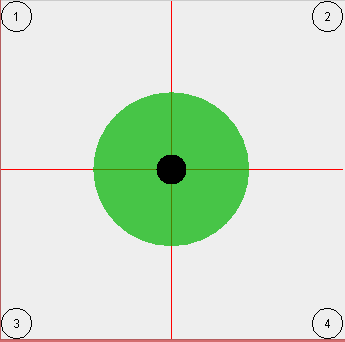
\includegraphics[scale=1]{image/jpanel1.png}
%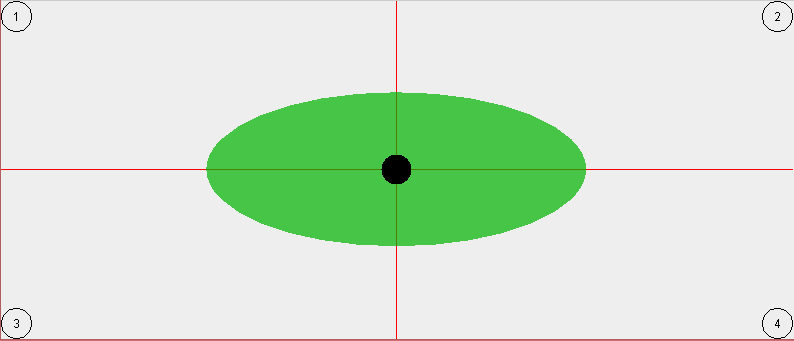
\includegraphics[scale=1]{image/jpanel2.png}
%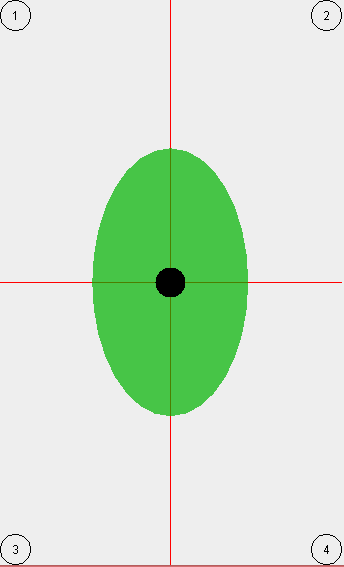
\includegraphics[scale=1]{image/jpanel3.png}
%\end{figure}

La mise à l'échelle correspond donc à exprimer les données de notre référentiel \guillemotleft ~réel \guillemotright\ dans le référentiel \guillemotleft\ Swing~\guillemotright\  servant à la visualisation dans le JPanel. 
L'idée est que, peut importe la forme du JPanel et les dimensions de la fenêtre, le barycentre, la deadzone et les pieds se comporte toujours de la même façon.
 Nous avons cherché à garantir que si l'utilisateur voit le barycentre sortir de la deadzone alors en réalité c'est bien parce que son centre de gravité sors de la deadzone et non à cause une mauvaise implémentation de l'interface graphique.
 
\begin{figure}[htbp]
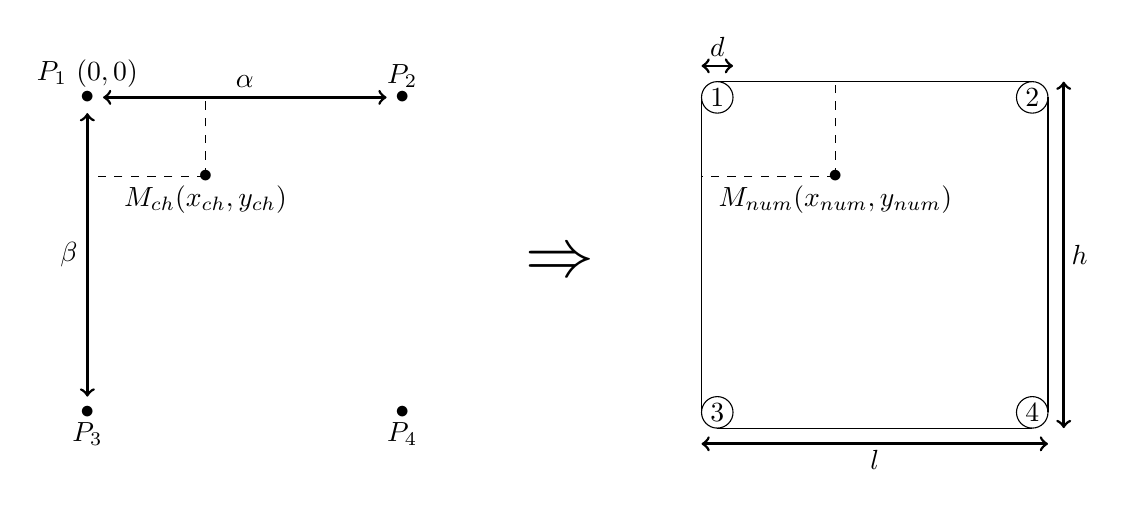
\begin{tikzpicture}
\coordinate (P1) at (0,4);
\coordinate (P2) at (4,4);
\coordinate (P3) at (0,0);
\coordinate (P4) at (4,0);
\coordinate (A) at (2,4);
\coordinate (B) at (0, 2);
\coordinate (ARR) at (6,1.6);
\coordinate (MCH) at (1.5, 3);

\draw[<->, line width=1pt] (0.2,4) -- (3.8,4);
\draw[<->, line width=1pt] (0,0.2) -- (0,3.8);
\draw (A) node[above] {$\alpha$};
\draw (B) node[left] {$\beta$};

\draw (P1) node[above] {$P_1\ (0, 0)$} node{$\bullet$};
\draw (P2) node[above] {$P_2$} node{$\bullet$};
\draw (P3) node[below] {$P_3$} node{$\bullet$};
\draw (P4) node[below] {$P_4$} node{$\bullet$};

\draw (MCH) node[below] {$M_{ch} (x_{ch}, y_{ch})$} node{$\bullet$};
\draw [-] [dashed] (MCH) -- (0,3);
\draw [-] [dashed] (MCH) -- (1.5,4);

\draw (ARR) node[above] {\Huge{$\Rightarrow$}};

\coordinate (S1) at (8, 4);
\coordinate (S2) at (12, 4);
\coordinate (S3) at (8, 0);
\coordinate (S4) at (12, 0);
\coordinate (D) at (8, 4.4);

\draw[<->, line width=1pt] (7.8,4.4) -- (8.2,4.4);
\draw (D) node[above] {$d$};

\draw (S1) circle (.2cm);
\draw (S2) circle (.2cm);
\draw (S3) circle (.2cm);
\draw (S4) circle (.2cm);

\draw (S1) node {$1$};
\draw (S2) node {$2$};
\draw (S3) node {$3$};
\draw (S4) node {$4$};

\draw [-] (8, 4.2) -- (12, 4.2);
\draw [-] (8, -0.2) -- (12,-0.2);
\draw [-] (7.8, 4) -- (7.8, 0);
\draw [-] (12.2, 4) -- (12.2, 0);

\draw[<->, line width=1pt] (12.4, -0.2) -- (12.4, 4.2);
\draw[<->, line width=1pt] (7.8, -0.4) -- (12.2, -0.4);

\draw (10, -0.6) node {$l$};
\draw (12.6, 2) node {$h$};

\coordinate (MNUM) at (9.5, 3);
\draw (MNUM) node[below] {$M_{num} (x_{num}, y_{num})$} node{$\bullet$};
\draw [-] [dashed] (MNUM) -- (7.8, 3);
\draw [-] [dashed] (MNUM) -- (9.5, 4.2);
\end{tikzpicture}
\caption{Le même point exprimé en deux référentiels : \textit{réel} (à gauche) et \textit{numérique} (à droite).}
\label{fig:visualisation_referentiels}
\end{figure}

Supposons une chaise à quatre pieds (voir la figure \ref{fig:visualisation_referentiels}), dont la largeur est $\alpha$ et la hauteur $\beta$.
 Supposons aussi que le JPanel a une hauteur $h$ et une largeur $l$. Notons $d$ le diamètre des cercles utilisés dans le panneau, c'est-à-dire le cercle qui représente le barycentre, et les cercles qui représentent les pieds de la chaise.
 Alors, la largeur et la hauteur de la chaise dans le panneau de visualisation sont :

\begin{equation}
\mathrm{largeur_{chaise}} = l - d
\end{equation}

\begin{equation}
\mathrm{hauteur_{chaise}} = h - d
\end{equation}

Dans le référentiel réel, les pieds sont représentés par des points tandis que dans le référentiel du JPanel ils sont représentés par des cercles. 
Soustraire $d$ aux dimensions du JPanel pour avoir les dimensions de la chaise dans le JPanel permettent d'assurer que nos cercles sont bien contenus dans celui-ci si on identifie les coins du JPanel aux pieds de la chaise.

Cependant, quand on passe à l'implémentation de ces formules, on fait face à une petite différence. 
Pour obtenir la hauteur et la largeur du JPanel, on utilise la méthode \texttt{$h$=getHeight()} et, respectivement, \texttt{$l$=getWidth()}).
Or, comme il est noté dans la documentation [REFERENCE BIBLIOGRAPHIQUE], ces méthodes nous donnent un nombre qui est un pixel trop grand. 
Nous devons donc le supprimer ce qui donner donc \texttt{$l$=getWidth()-1} et \texttt{$h$=getHeight()-1}.
On a donc finalement la hauteur et largeur de la chaise dans le JPanel :

\begin{center}
$\mathrm{hauteur_{chaise}}$  = getHeight() - 1 - diamètre\\
$\mathrm{largeur_{chaise}}$ = getWidth() - 1 - diamètre
\end{center}

A l'aide d'un produit en croix, nous pouvons désormais mettre à l'échelle les dimensions de la chaise car on connais les dimensions de la chaise dans la réalité (dans l'objet Chaise) et les dimensions de la chaise dans le JPanel.
Les dimensiosn que nous avons calculé jusqu'à présent nous permettent donc de faire le lien entre la position d'un point dans la réalité (le barycentre par exemple) et sa représentation dans le JPanel.
Si on donne les coordonnées cartésiennes d'un points réel ($x_{Chaise}$,$y_{Chaise}$) on peut trouver où le dessiner dans le JPanel à l'aide des coordonnées ($x_{JPanel}$,$y_{JPanel}$) à l'aide des equations \eqref{eqn:form_ref_hor} et \eqref{eqn:form_ref_vert}.

\begin{equation}
\label{eqn:form_ref_hor}
x_{JPanel} = x_{Chaise}\ \ \frac{\mathrm{largeur}}{\alpha} + \frac{d}{2}
\end{equation}

\begin{equation}
\label{eqn:form_ref_vert}
y_{JPanel} = y_{Chaise}\ \ \frac{\mathrm{hauteur}}{\beta} + \frac{d}{2}
\end{equation}

où($x_{Chaise}$,$y_{Chaise}$) est un point quelconque dans le référentiel de la chaise (c'est-à-dire le référentiel \guillemotleft ~réel~\guillemotright ), et ($x_{JPanel}$,$y_{JPanel}$) est le même point, exprimé dans le référentiel du JPanel.

En somme, les méthodes \texttt{scaleX(double xChaise)} et \texttt{scaleY(double yChaise)} permettent de dessiner n'importe quel élément (que ce soit le barycentre ou la deadzone) avec la certitude que l'échelle est respectée peu importe la taille de fenêtre.

Une fois qu'on a décrit la partie calculatoire qui assure le bon fonctionnement du panneau de visualisation, nous allons passer à la description des éléments interactifs de l'interface graphique. 
Nous avons déjà parlé brièvement du JPanel que nous avons utilisé en tant que zone de dessin. Nous allons maintenant voir qu'il est aussi utilisé en tant que conteneur.

Nous avons utilisé les objets \texttt{JFrame} et \texttt{JPanel} pour séparer la fenêtre de notre application en deux.
Nous communiquons à l'utilisateur que la partie gauche, à savoir le panneau de visualisation, va afficher des informations relatives à la qualité de la posture assise, alors que la partie droite va lui permettre de contrôler les paramètres du détecteur de posture.
 Finalement, en haut se trouve un menu construit à partir d'un objet \texttt{JMenu}, qui permet d'enregistrer ou de charger une chaise.

Ensuite, en utilisant deux objets \texttt{JButton} et un objet \texttt{JComboBox}, nous avons créé la partie \textit{communication} du panneau de contrôle.

 Le \texttt{JComboBox} est tout simplement une liste contenant tous les ports série disponible sur la machine et récupérable grâce à la librairie JSerialComm.
Les \texttt{JButton} sont des boutons, permettant de se connecter ou se déconnecter du port choisi (voir figure \ref{fig:app_pc_comms}). Évidemment, nous avons mis en place des mécanismes pour que les boutons \guillemotleft ~Connexion \guillemotright\ et \guillemotleft\ Déconnexion~\guillemotright\ soient actifs seulement s'il le faut.
Par exemple, l'utilisateur ne doit pas être capable de cliquer sur \guillemotleft ~Déconnexion~\guillemotright\ s'il n'est pas connecté au préalable. 
Ce fonctionnement permet de faciliter l'apprentissage du logiciel et de limiter les bugs d'interaction avec l'utilisateur.

\begin{figure}[htbp]
\begin{center}
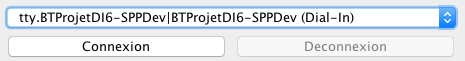
\includegraphics[width=12cm]{image/app_pc_comms}
\end{center}
\caption{Les contrôles de communication dans l'application PC.}
\label{fig:app_pc_comms}
\end{figure}

En dessous de ces trois éléments se trouvent trois autres boutons, qui ne concernent pas la connexion avec l'Arduino, mais les paramètres du détecteur de posture : 
\begin{itemize}
\item Le bouton \guillemotleft ~Tare~\guillemotright\ permet de faire le zéro des capteurs.
\item Le bouton \guillemotleft ~Config chaise~\guillemotright\ permet de configurer les paramètres de la chaise (c'est-à-dire le nombre des pieds et leurs positions)
\item Le bouton \guillemotleft ~Calibrer la zone~\guillemotright\ permet de centrer la deadzone à la position actuelle du barycentre (voir figure \ref{fig:app_pc_chaise}). Ce dernier bouton est important, car il permet à l'utilisateur de contrôler la position de la zone optimale. 
Il est à noter que celle-ci n'est pas forcément au centre de la chaise, puisqu'elle dépend de la forme et de la posture optimale sur la chaise en question.
\end{itemize}

Enfin, un objet \texttt{JSlider} permet de contrôler la taille de la deadzone (voir figure \ref{fig:app_pc_chaise}). 
Le diamètre de la deadzone est libre et il conviendrait de consulter un ergothérapeute pour connaître la limite dans laquelle on autorise des modifications de posture.

Cependant, il va de soi que plus la deadzone est petite, plus le détecteur sera sensible.

%Il est tout à fait possible d'avoir une deadzone dont le diamètre est égal à la plus petite dimension de la chaise; toutefois il est fortement conseillé d'avoir la deadzone la plus petite possible, afin que le détecteur soit plus précis.

\begin{figure}[htbp]
\begin{center}
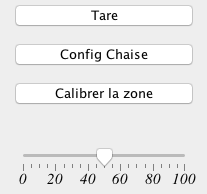
\includegraphics[width=6cm]{image/app_pc_chaise}
\end{center}
\caption{Les contrôles de configuration de la chaise.}
\label{fig:app_pc_chaise}
\end{figure}

Pour conclure, notre choix d'utiliser exclusivement des éléments \texttt{Swing} pour construire l'interface graphique repose sur le fait que cette librairie est très bien documentée et supportée en ligne.
Les documentations nous ont permis de résoudre tous les problèmes que nous avons rencontrés et de rendre notre interface graphique fonctionnelle.


\chapter*{Conclusion}


Au travers de ce projet de construction d'un correcteur de posture assise, nous avons montré que nous étions capable de faire preuve d'initiative et de créativité.
Nous avons démontré notre capacité à nous approprier le fonctionnement du micro-contrôleur Arduino et nous avons réussi à dimensionner et interfacer correctement des capteurs avec celui-ci.
Finalement, à l'aide d'un Arduino et de capteurs de forces récupérés sur un pèse-personne électronique on peut créer un correcteur de posture assise.
Notre logiciel fonctionnant à la fois sur PC et sur un appareil Android est un agrément non négligeable et permet de rendre l'utilisation du correcteur de posture simple et ludique.

En 12 séances de travail, nous avons réussi à étudier et concevoir un correcteur de posture alors que nous n'avions jamais manipulé de micro-contrôleur auparavant.
Heureusement, nos projets personnels et polytech précédent nous avaient permis d'acquérir d'excellentes bases en programmation (notamment JAVA) et les nouveautés se sont surtout situés au niveau du micro-contrôleur et de l'électronique. 

Nous avons réussi a surmonter ces nouveautés en électronique et informatique embarqué et c'est avec fierté et enthousiasme que nous vous présentons notre prototype.

Afin de garder l'esprit ouvert sur le perfectionnement de ce prototype, nous avons réfléchit à des améliorations telles que:

%Notre prototype actuel bien que fonctionnel pourrait subir des améliorations auxquelles nous avons réfléchit:

\begin{itemize}
\item Réduction de sa taille notamment en passant sur une version miniature de l'Arduino Uno (Arduino Pro Mini);
\item Incruster les capteurs directement dans les pieds de la chaise pour plus de maniabilité;
\item L'amélioration de l'autonomie en modifiant la gestion des amplificateurs et l'ajout d'une fonction de veille lorsque personne n'est assis sur la chaise;
\item Ajout de LEDs RGB changeant de couleur et de vibreurs au niveau du plateau de l'assise pour notifier l'utilisateur en cas de mauvaise assise;
\item Ajout de la possibilité de choisir un mode graduel de notification (LED pour les petites sorties de la zone, Vibreur ensuite et Son pour les sorties extrêmes de la zone);
\item Ajout de nouvelles fonctions de paramétrage (couleurs de LEDs et vibreurs) dans l'application mobile.
\end{itemize}

Ces améliorations (réalisables avec plus de temps) permettraient de rendre l'utilisation du correcteur de posture transparente et permettraient peut-être d'aboutir à un produit commercialisable.

%Avec ce rapport nous espérons que vous avez eut l'opportunité d'apprécier notre travail.


\chapter{SOURCES}
BROUILLON BIBLIOGRAPHIE
\url{https://www.arduino.cc/}
\url{http://www.ntu.edu.sg/home/ehchua/programming/java/J4b_CustomGraphics.html}






%% === COMPTES RENDUS ===
\weeklyreport{11/01/2017}{
Séance 1:
Expérimentation et choix techniques:
\begin{itemize}
\item Installation IDE Arduino + pilotes
\item Création du dépôt Github
\item Premier code Arduino: faire clignoter la LED intégrée
\item Acquisition du capteur de pression et affichage moniteur série
\item Dialogue JAVA série via jSerialComm entre Arduino et PC
\end{itemize}
}

\weeklyreport{18/01/2017}{
Séance 2:
Travail sur le matériel:
\begin{itemize}
\item Branchement de 3 potentiomètres + un FSR sur l'Arduino
\item Recherche de capteurs capable de mesurer des force plus grandes
\end{itemize}
Programmation:
\begin{itemize}
\item Mise en place du protocole de communication des données
\item Programmation d'une première interface graphique avec JAVA Swing pour visualiser la chaise
\item Première vidéo de fonctionnement du programme
\end{itemize}
}

\weeklyreport{25/01/2017}{
Séance 3:
Travail sur le matériel:
\begin{itemize}
\item Démontage d'une balance électronique pour étudier les capteurs de charges
\item Mesure des résistances des capteurs de charges et création d'un pont WheatStone
\item Tentative de mesure du pont wheatstone (échec)
\item Ajout du Shield Bluetooth sur l'Arduino
\item Test d'alimentation de l'Arduino via une batterie portable
\end{itemize}
Programmation:
\begin{itemize}
\item Modification du code de l'Arduino pour recevoir des données depuis le PC
\item Ajout du code de prise en charge du Shield Bluetooth
\end{itemize}
}

\weeklyreport{01/02/2017}{
Séance 4:
Programmation:
\begin{itemize}
\item Démarrage du développement de l'application Android sur Android Studio
\item Ajout de fonctionnalité de paramétrage de la chaise sur PC
\end{itemize}
}

\weeklyreport{08/02/2017}{
Séance 5:
Programmation:
\begin{itemize}
\item Ajout de la fonction de paramétrage d'une "deadzone" dans laquelle on dit que la posture assise est correcte.  Un cercle vert indique la zone de confort. Les informations à propos de cette zone sont stockés dans l'objet Chaise conçu pour effectuer tout les calculs.
\item Corrections de bugs dans l'application Android. Amélioration des performances.
\item Modification du nom bluetooth du shield Arduino (BTProjetDI6)
\end{itemize}
}

\weeklyreport{15/02/2017}{
Séance 6:
Programmation:
\begin{itemize}
\item Retour au tableau blanc, correction de bugs introduits par la fonctionnalité de deadzone
\item Ajout de fonctionnalité de sauvegarde et chargement de l'objet chaise.
\end{itemize}
}

\weeklyreport{08/03/2017}{
Séance 7:
Programmation:
\begin{itemize}
\item Finalisation de la sauvegarde et du chargement de la chaise sur PC
\item Début de l'implémentation de la fonction de chargement sur Android
\item Modification du code de l'Arduino pour prendre en charge les amplificateurs HX711
\end{itemize}
Matériel:
\begin{itemize}
\item Récupération de 4 cellules de charges
\item Fabrication des ponts wheatstones fonctionnels
\item Connexion de 3 amplificateurs HX711 pour utiliser les capteurs de charges
\end{itemize}
}

\weeklyreport{15/03/2017}{
Séance 8:
Programmation:
\begin{itemize}
\item Modification du parser pour l'objet chaise (correction de bugs et modification du fonctionnement, la sérialisation ne marchait pas bien)
\item Modification du code de l'Arduino pour adapter la mesure des capteurs de charges (réduire le bruit)
\end{itemize}
}

\weeklyreport{22/03/2017}{
Séance 9:
Programmation:
\begin{itemize}
\item Refactoring du code d'enregistrement 
\item Modification de la description de la deadzone (on utilise le ratio maintenant)
\item Ajout des boutons Tare sur PC et Android
\item Prise en charge de la Tare sur l'Arduino
\end{itemize}
Matériel:
\begin{itemize}
\item Design de cales pour les capteurs de charges sur AutoCad
\item Réalisation de cales en bois MDF pour les capteurs de charges
\end{itemize}
Première simulation:
On a posé une chaise sur les capteurs et on a posé un sac sur celle-ci après avoir fait la calibration. 
On arrive bien à détecter la position du sac.
}

\weeklyreport{29/03/2017}{
Séance 10:
Programmation:
\begin{itemize}
\item Amélioration de l'acquisition des valeurs dans le programme Arduino
\end{itemize}
Matériel:
\begin{itemize}
\item Changement des fils de connexion des capteurs de charges
\item Ajout d'une protection mécanique des fils avec de la gaine thermo-rétractable
\end{itemize}
Rédaction du rapport de projet
}

\weeklyreport{05/04/2017}{
Séance 11:
Matériel:
\begin{itemize}
\item Recherche d'une plaque à poser sur les capteurs de charge pour les protéger et éviter un contact direct avec les pieds de la chaise
\item Dimension de la plaque $60 \times 60$ cm ou $65 \times 65$ cm.
\end{itemize}
Rédaction du rapport de projet
Prise de photos pour le rapport de projet
}

\weeklyreport{26/04/2017}{Rapport seance 12}


\end{document}


